\documentclass[a4paper,fleqn]{cas-sc}
\usepackage[numbers,sort&compress]{natbib}
\usepackage{amsmath,amssymb,microtype,booktabs,array,tikz}
\microtypesetup{expansion=false}
\usepackage{placeins}
\usetikzlibrary{arrows.meta,positioning,calc}
\hypersetup{hidelinks}
\setlength{\tabcolsep}{4pt}
\setlength{\emergencystretch}{2em}
\graphicspath{{generated/}}
\ExplSyntaxOn
\cs_set:Npn \__first_footerline: {\small\rmfamily Manuscript~draft}
\ExplSyntaxOff
\let\printorcid\relax
% CAS puts the keyword box in a zero-width overlay; provide stretch to avoid
% a spurious overfull-box diagnostic without changing its visible placement.
\ExplSyntaxOn
\RenewDocumentEnvironment{Abstract}{o}
{
  \group_begin:
  \IfNoValueTF{#1}{}{\tex_gdef:D\abstractname{#1}}
  \parindent=0pt
  \box_if_empty:NTF\g_stm_key_box{\leftskip=.35\textwidth}
  {
    \dim_gset:Nn\l_tmpa_dim{\box_ht:N\g_stm_key_box}
    \dim_gadd:Nn\l_tmpa_dim{\box_dp:N\g_stm_key_box}
    \leftskip .35\textwidth
    \hspace*{-.35\textwidth}
    \noindent\hbox_to_wd:nn{0pt}{\box\g_stm_key_box\hss}
    \skip_vertical:n{-\l_tmpa_dim}
  }
  \noindent\abstractname\par
  \skip_vertical:n{-4pt}
  \noindent\rule{.65\textwidth}{.2pt}\par\footnotesize
  \ignorespaces\everypar{\parindent=1.5em}
}{\par\group_end:}
\ExplSyntaxOff
\raggedbottom
\begin{document}
\let\WriteBookmarks\relax
\shorttitle{Observation-anchored event editing for fault diagnosis}
\shortauthors{R. Cao and J. Liu}
\title[mode=title]{Observation-anchored event-mechanism editing for fault diagnosis under unseen operating conditions}
\author[1]{Runze Cao}
\author[1]{Jie Liu}
\cormark[1]
\affiliation[1]{organization={School of Reliability and Systems Engineering, Beihang University (BUAA)},city={Beijing},country={China}}
\cortext[1]{Corresponding author.}
% Add the corresponding author's confirmed email with \ead{...} before submission.
% Funding, CRediT and competing-interest statements require the authors' confirmation.
\begin{abstract}
Operating-condition changes modify the timing and excitation strength of fault-related vibration events, while measured signals also contain structural responses and background components. Enforcing invariance on the entire observation can therefore suppress information useful for diagnosis. This paper proposes observation-anchored event-mechanism editing for domain-generalized fault diagnosis. A source-only sparse analyzer estimates events in a finite response dictionary. The editor changes event locations and effective impulse strength while retaining the response kernels and the remainder of each measured observation. Factual and edited source views train a shared log-spectrum classifier with instance normalization and Mixup. Deployment requires only a vibration window and introduces no additional analysis branch. Experiments cover 27 multi-source tasks on Paderborn bearings, PHM09 gearboxes and JNU bearings, with ten random runs per task. The proposed recipe achieves window accuracies of $83.12\pm0.94\%$, $71.98\pm0.95\%$ and $99.67\pm0.17\%$, respectively. Its dataset-equal accuracy exceeds matched instance normalization and Mixup by 0.80 percentage points and the unedited-bank control by 0.79 points. Same-rate timing-only and global-moment controls distinguish the contribution of selective event editing. On PU, recording-level fault-to-healthy errors decrease from 10.41\% to 9.12\%; on PHM09, the run-to-run standard deviation decreases from 1.85 to 0.95 points. Comparisons with strong alignment baselines, checkpoint selection and a single-source extension characterize the conditions under which the editor provides useful diagnostic improvements.
\end{abstract}
\begin{keywords}
Fault diagnosis \sep Domain generalization \sep Mechanism intervention \sep Sparse event analysis \sep Vibration signals
\end{keywords}
\maketitle

\section{Introduction}
Vibration-based fault diagnosis supports condition monitoring and maintenance by identifying changes in the health state of rotating machinery. Deep diagnostic models can learn discriminative patterns from labeled measurements, but their deployment often involves speeds and loads that differ from those observed during training. A change in operating condition modifies both the excitation of a fault and the way its response appears in a measurement. Consequently, a classifier may fail even when the target fault categories are represented in its training data.

Domain generalization (DG) addresses this setting by training on observed source conditions and evaluating on an unseen target condition. Unlike domain adaptation, it does not require target observations during training. Recent research has developed alignment, contrastive, augmentation and causal learning strategies for this purpose \cite{zhao2024,chen2025}. The application-oriented study of Zhao et al.~\cite{zhao2024} also shows why empirical risk minimization (ERM), evaluation protocols and the distinction between condition and machine transfer matter when assessing these methods. A useful diagnostic method must demonstrate its increment under the actual information available at deployment.

Causal approaches offer a way to organize this problem around factors that generate the measurements. CIS2N constrains feature dependence and changes between intervention pairs \cite{cis2n}. PC3Net combines prior features, causal-feature learning and collaborative classification for single-source generalization \cite{pc3net}. Anti-causal learning studies the causes of simulated domain shifts \cite{antic2024}. These approaches place useful structure on representation learning. However, operating conditions can affect fault-bearing components themselves: impact spacing, impulse strength and resonance response need not change together. A restriction on an entire representation or waveform does not explicitly distinguish these actions.

This observation motivates a different intervention location. Rather than estimate a condition branch and remove it, we change a specified part of the source observation while retaining the remaining measured signal. Under a convolutional event model, moving an excitation changes its occurrence time without necessarily changing the response kernel. In contrast, dilating an entire waveform moves the excitation and changes the oscillations within its response. Moreover, a sparse analysis model cannot be expected to explain every useful component of a real measurement. Replacing the complete signal with its reconstruction would discard that unexplained information.

We propose observation-anchored event-mechanism editing to address these two issues. A numerical source analyzer estimates event coefficients and finite response kernels. The editor moves the estimated events, scales their effective impulse strength according to a fixed rule, and adds the change to the original measurement. The response kernels and the observation-anchored remainder are retained. This construction supplies edited source queries to a conventional diagnostic network; the analyzer is absent from deployment. The method is causal in its motivation and intervention specification within a working signal-generation model. Its learning contribution is evaluated by matched controls that separate event timing, impulse strength, global amplitude statistics and bank sampling.

The main contributions are as follows.
\begin{enumerate}
\item An observation-anchored event operator changes event locations and effective impulse strength without dilating the response kernels or replacing the unexplained measured signal. The operator recovers the factual observation exactly at unit rate.
\item A source-only learning procedure integrates the editor with factual supervision and feature-space Mixup. Source analysis is performed offline, and the deployed classifier uses a single vibration window without target speed, a paired recording or an inverse solver.
\item A ten-run evaluation across 27 cross-condition tasks establishes the operator's increment over matched strong controls and examines recording-level errors and repeatability. Timing-only, impulse-only, moment-matched and exposure controls identify which parts of the construction contribute, while a six-direction single-source extension tests its behavior under reduced source coverage.
\end{enumerate}

\section{Related work}
\subsection{Domain generalization for fault diagnosis}
DG methods seek a diagnostic rule that transfers beyond the source distributions. Distribution alignment encourages shared feature statistics; domain-adversarial learning discourages source-domain discrimination; contrastive methods use labels to organize inter-domain relationships. CCDG, for example, promotes class-conditioned agreement using a contrastive objective \cite{ccdg}. Deep CORAL and domain-adversarial learning provide established alignment objectives \cite{coral,dann}; in a DG setting these objectives can be applied among source domains without supplying target observations.

DG also includes distinct information settings. Multi-source DG learns from several observed conditions, whereas single-source DG must construct useful variation from one condition. PC3Net combines statistical prior features and learned causal features in the latter setting \cite{pc3net}. More recent semi-supervised DG addresses incomplete source labels: the two-stage network of Cui et al.~\cite{cui2026} combines pseudo-label construction, feature augmentation and regularized generalization learning. These settings should be distinguished when comparing results. The main study here is supervised multi-source cross-condition diagnosis; the JNU single-source extension is reported separately.

\subsection{Causal representations and mechanism-guided construction}
CIS2N formulates causal independence and sparse feature shifts, implemented through random Fourier feature covariance and a sparse-shift penalty \cite{cis2n}. MOCD combines sample matching with dual representations intended to distinguish class-related and domain-related information \cite{mocd}. CFDCR integrates causal representation learning with adversarial adaptation and uses unlabeled target data \cite{cfdcr}; it is therefore a related causal approach with a different information setting. These works motivate structural constraints but differ from an explicit edit of an estimated source-signal component.

Physical source construction offers another route. Pang et al.~\cite{pang2024} combine analytical fault vibration with measured normal backgrounds. Shi et al.~\cite{shi2024} combine semi-physical simulation and contrastive decoupling under speed variation. Physics-guided counterfactual causal learning uses counterfactual regularization and an order-interaction network for single-source cross-machine diagnosis \cite{pcr2026}. Thus physical synthesis, measured background and counterfactual learning are established ideas. The present contribution is more specific: each edit retains the remainder of its own labeled observation and changes the estimated event clock while holding the response kernels fixed.

\begin{table}[pos=htbp]
\centering\small
\caption{Relationship to representative mechanism-guided approaches. This comparison concerns constructions and information requirements.}
\label{tab:position}
\begin{tabular}{>{\raggedright\arraybackslash}p{.19\linewidth}>{\raggedright\arraybackslash}p{.34\linewidth}>{\raggedright\arraybackslash}p{.35\linewidth}}
\toprule
Approach & Main learning action & Distinction of the present method\\
\midrule
CIS2N \cite{cis2n} & Independence and sparse shifts of learned features & Edits an estimated signal component before feature extraction.\\
PC3Net \cite{pc3net} & Prior/causal feature collaboration in single-source DG & Uses measured-context event edits and a single deployed classifier.\\
MOCD \cite{mocd} & Matched pairs and class/domain representation branches & Keeps the measured remainder without a deployed domain branch.\\
Fault-model-driven DG \cite{pang2024} & Simulated faults with measured normal backgrounds & Retains the remainder of each labeled observation, including faulty recordings.\\
PCR-OIPN \cite{pcr2026} & Physics-guided counterfactual learning and order interaction & Edits event occurrence with fixed kernels; deployment requires no target speed.\\
Whole-waveform scaling & Dilation of events, responses and background & Moves estimated events while retaining response shape and observed remainder.\\
\bottomrule
\end{tabular}
\end{table}

Table~\ref{tab:position} summarizes this distinction. The numerical sparse solver \cite{fista}, instance normalization (IN) \cite{in} and Mixup \cite{mixup} are adopted components. The proposed method concerns their use with an observation-anchored event intervention, and the experiments isolate this intervention from the benefits of the surrounding classifier recipe.

\section{Proposed method}
\label{sec:method}
\subsection{Problem formulation}
Let $\mathcal D_s=\{(w_i,y_i,d_i)\}_{i=1}^{N_s}$ contain labeled vibration
windows from the observed source conditions, where $y_i\in\{1,\ldots,K\}$
is a fault label and $d_i\in\{1,\ldots,D\}$ identifies a source condition.
The objective is to train a classifier that diagnoses an unseen condition
using only its vibration window. Target signals, labels, rotational speeds,
and target-batch statistics are not inputs to the training algorithm.
Recorded source speeds and sampling rates are used by an offline source
analyzer. The analyzer and its source partners are not needed at deployment.

The fixed two-rate implementation is denoted Q2.
The proposed training construction acts on source observations before
feature extraction. It modifies the timing and effective impulse strength
of an estimated event component while retaining the response kernels and the
unexplained part of the observation. A factual training branch remains in
the classification objective throughout training.

Figure~\ref{fig:framework} summarizes the offline analyzer, source-training
path and deployment path. The editor changes the training distribution;
it adds no inverse solver or source-matching step to deployment.
\begin{figure}[pos=htbp]
\centering
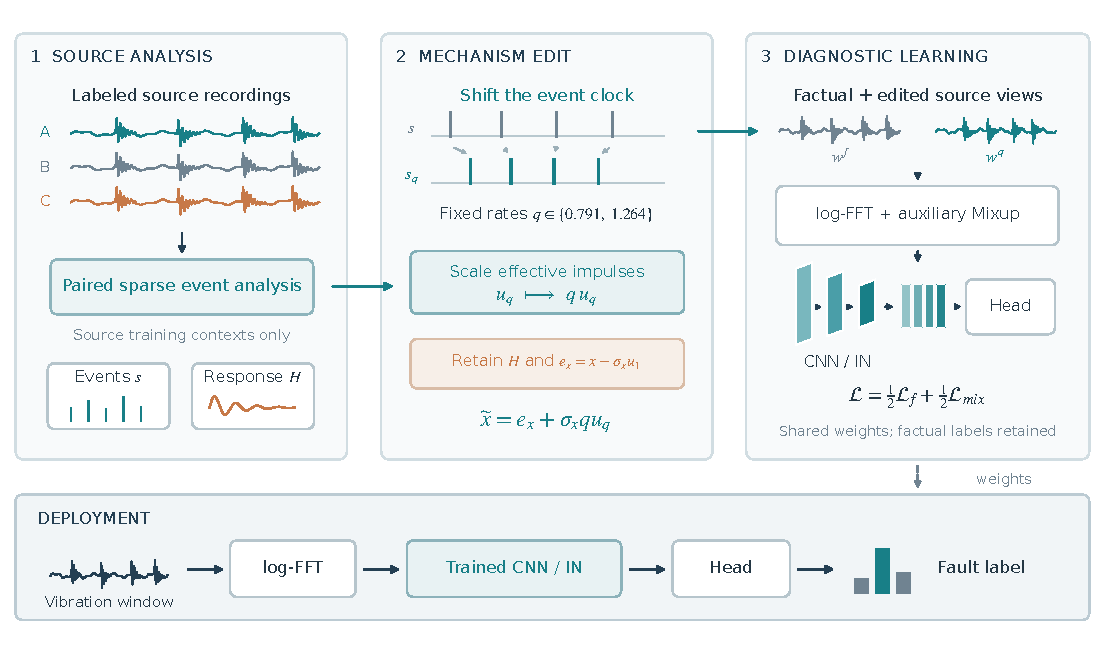
\includegraphics[width=\linewidth]{framework_publication.pdf}
\caption{Observation-anchored event-mechanism editing. Source analysis estimates events and response kernels. The intervention changes event timing and effective strength while retaining the response and observation-anchored remainder. Factual and edited views train one shared network; deployment uses the frontend and classifier only. Traces and feature blocks illustrate the processing stages and are not experimental measurements.}
\label{fig:framework}
\end{figure}


\subsection{Source event analysis}
For a source context $x\in\mathbb R^N$, write
$\bar x=(x-\mu_x)/\sigma_x$, where $\mu_x$ and $\sigma_x>0$ are its saved
source mean and scale. The source analyzer fits a nonnegative event model
together with harmonic and stationary terms:
\begin{equation}
 \bar x_j=H_js_j+A_jb_j+Fc_j+\epsilon_j,\qquad s_j\geq0,
 \quad j\in\{1,2\}.
 \label{eq:analysis}
\end{equation}
Here $j$ indexes two legal source contexts, $H_j$ is a finite convolution
dictionary, $A_j$ contains the first four recorded shaft harmonics, and $F$
contains stationary sinusoidal candidates estimated from the source pair.
Each response dictionary contains four source spectral carrier candidates,
three decay values, and four phases, giving 48 response modes per context.
These modes are analysis kernels; they do not mask frequency bands in the
classifier input.

The sparse inverse minimizes a squared reconstruction term with
nonnegative $\ell_1$ penalties on $s_j$ and group penalties on the sinusoidal
coefficients:
\begin{equation}
 \min_{\substack{s_1,s_2\geq0\\b_1,b_2,c_1,c_2}}
 \frac12\sum_{j=1}^{2}
 \|\bar x_j-H_js_j-A_jb_j-Fc_j\|_2^2
 +\sum_{j=1}^{2}\lambda_{s,j}\|s_j\|_1
 +\lambda_b\|B\|_{2,1}
 +\lambda_c\|C\|_{2,1}.
 \label{eq:inverse}
\end{equation}
A group in $B$ or $C$ contains the corresponding sine and cosine
coefficients across the two source contexts. Fixed proximal iterations
produce the offline coefficients and kernels used to construct the source
bank using accelerated proximal updates \cite{fista}. The classifier does not
backpropagate through this numerical inverse.

Source labels are used when selecting same-class source pairs, even though
Eq.~\eqref{eq:inverse} has no classification loss. The current PU pairing
also preserves the recorded bearing identity. A verified entity identity
is not assumed for PHM or JNU. Both contexts must belong to the current
source-training role; a source-validation or target context cannot serve
as an analysis partner.

\subsection{Observation-anchored mechanism editing}
For one analyzed context, let $s_b[n]$ denote its event coefficients and
$h_b$ its finite response kernels. A kernel is zero outside $[0,L-1]$.
Using the context center $m=(N-1)/2$, define a relative event-rate
transformation
\begin{equation}
 u_q[t]=\sum_{b=1}^{48}\sum_{n=0}^{N-1}
 s_b[n]\,
 h_b\!\left(t-m-\frac{n-m}{q}\right),\qquad q>0.
 \label{eq:render}
\end{equation}
Thus event locations move from $n$ to $m+(n-m)/q$ while the response
shape remains fixed. Fractional lags are evaluated from the same finite
analytic kernel used at $q=1$; they are not created by resampling the
complete recorded waveform. The implementation evaluates $u_1$ and
$u_q$ using the same float64 rendering definition and checks context support
before extracting a query window.

Define the observation-anchored remainder by
\begin{equation}
 e_x=x-\sigma_xu_1 .
 \label{eq:remainder}
\end{equation}
The coupled edit is
\begin{align}
 \mathcal T_q(x)
   &=e_x+\sigma_xq u_q \nonumber\\
   &=x+\sigma_x(q u_q-u_1).
 \label{eq:edit}
\end{align}
The remainder includes the source mean and all components not represented
by $\sigma_xu_1$. It is retained rather than assigned to a disposable
condition branch. Consequently, the method does not require every
condition-dependent feature to be estimated and subtracted.

The relative rate $q$ changes event density and the factor $q$ in
Eq.~\eqref{eq:edit} changes effective event impulse strength. The fixed
coupling rule scales effective impulses linearly with relative rate.
Waveform energy also depends on event overlap, finite support and the
retained remainder.

The implementation returns $\mathcal T_1(x)=x$ exactly. For other values,
the edited query is obtained by cropping the transformed context,
$w^{\,q}=P_r\mathcal T_q(x)$, using the original query location $r$.
No new response or event inverse is fitted for each edit. The current
Q2 recipe samples the two fixed values
\begin{equation}
 q\in\left\{\exp\!\left(-\frac{\log(1.5)}{\sqrt3}\right),
                 \exp\!\left(\frac{\log(1.5)}{\sqrt3}\right)\right\}
       \approx\{0.791286,\;1.263765\}
 \label{eq:q}
\end{equation}
with equal probability. These factors are the same across datasets and are
not chosen from a target rotational speed.

The intervention variables in this event model are event location and
effective impulse strength, with the response and remainder held fixed.
Its utility is tested by matched timing-only, amplitude-only,
global-moment and unedited-bank controls.

The causal motivation is expressed within this event-generation model.
Writing $x=\sigma_x\mathcal H(s)+e_x$, the action changes the estimated
event locations and impulses, while the analyzed response $\mathcal H$ and
observation term $e_x$ are held fixed. Keeping the training label assumes that
the chosen local event changes preserve the diagnostic category. This is a
modeling assumption tested through the learning experiments; it does not follow
from reconstruction accuracy alone. Effective impulses can vary with operating
conditions without changing fault location, but the linear coupling in
Eq.~\eqref{eq:edit} is a fixed augmentation rule rather than a universal
load--speed law. The construction therefore specifies which mechanism is
intervened on without assigning every remaining signal component to a
non-causal branch.

\begin{samepage}
The distinction from waveform time scaling follows directly from the
kernel model. Set the time origin at the context center and write
$\tau_n=n-m$. The event edit and a dilation of the original modeled
component then give
\begin{align}
 v_q(t)&=\sum_{b,n}s_b[n]h_b\!\left(t-\frac{\tau_n}{q}\right),
 \label{eq:centered-edit}\\
 v_1(qt)&=\sum_{b,n}s_b[n]h_b\!\left(q\left[t-\frac{\tau_n}{q}\right]\right).
 \label{eq:waveform-dilation}
\end{align}
\end{samepage}
Both move event centers to $\tau_n/q$. Waveform dilation also scales
the time coordinate inside each response kernel. Q2 preserves the
response shape and scales effective impulse strength separately by $q$
in Eq.~\eqref{eq:edit}. These identities concern the continuous kernel
model; subsequent sampling and finite-query cropping produce the training
inputs. The harmonic and stationary terms retained in $e_x$ keep their
observed coordinates, so $q$ parameterizes an edit of the fitted event clock.

\begin{figure}[pos=htbp]
\centering
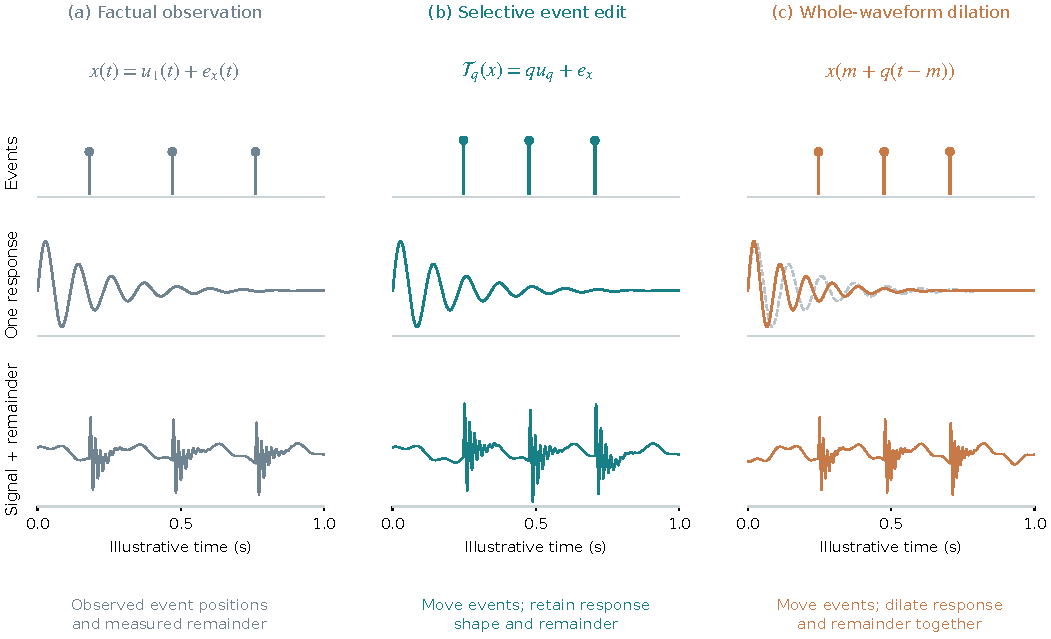
\includegraphics[width=.94\linewidth]{generated/mechanism_publication.pdf}
\caption{Analytic illustration of the operator distinction. Columns show the same three synthetic events under the factual model,
selective editing and whole-waveform dilation. Rows display events, one response
and the resulting observation; dashed traces indicate the original response
or retained background. The illustration uses $q=1.264$ and unit source scale. Q2 moves event centers and scales their impulses while preserving
the response and measured-context term. Whole-waveform dilation also changes
kernel oscillations and background coordinates. This illustration explains
the construction; it is not a measured-signal or classification experiment.}
\label{fig:mechanism}
\end{figure}

\subsection{Classification and feature-space Mixup}
A deterministic frontend $\Phi$ maps each factual or edited query to
$\log(1+|\operatorname{rFFT}(w)|)$, followed by linear interpolation to
2048 frequency positions. A shared convolutional encoder, channel-wise
instance normalization over the feature position axis, and classification
head produce the logits $f_\theta(\Phi(w))$.
Raw-valued queries enter this frontend; the context normalization used by the
offline analyzer is separate from the classifier input transformation.

Training samples are balanced over source-condition and class cells.
For each balanced slot $i$, a factual window $w_i^f$ is drawn from the full
source-training pool and a bank context/query $(x_i^b,r_i)$ is independently
drawn from the same condition and class. They need not come from the same
recording. Their labels agree because of the balanced slot construction;
this is not a requirement to classify one recording using another at test
time.

For a binary edit mask $M_i$, construct the auxiliary feature
\begin{equation}
 a_i =
 \begin{cases}
  \Phi(P_{r_i}\mathcal T_{q_i}(x_i^b)), & M_i=1,\\
  \Phi(w_i^f), & M_i=0 .
 \end{cases}
 \label{eq:aux}
\end{equation}
The mask is sampled with probability $1/2$. At each class and within-cell
position it is shared across source conditions, so that edit activation
does not introduce a different condition-wise sampling rule.
The same sampler and edit-direction streams are used for matched controls.

Mixup acts on the auxiliary features after the log-FFT frontend.
For a batch permutation $\pi$ and a shared
$\lambda\sim\operatorname{Beta}(0.2,0.2)$, let
\begin{equation}
 \widetilde a_i=\lambda a_i+(1-\lambda)a_{\pi(i)} .
 \label{eq:mix}
\end{equation}
The loss combines factual and mixed classification risks:
\begin{align}
 \mathcal L(\theta)
  ={}&\frac{1}{2B}\sum_{i=1}^{B}
       \ell(f_\theta(\Phi(w_i^f)),y_i)\nonumber\\
   &+\frac{1}{2B}\sum_{i=1}^{B}
       \big[\lambda\ell(f_\theta(\widetilde a_i),y_i)
       +(1-\lambda)\ell(f_\theta(\widetilde a_i),y_{\pi(i)})\big],
 \label{eq:loss}
\end{align}
where $\ell$ is cross-entropy.

The network forward concatenates three copies of the factual batch and
three copies of the same mixed batch. Each of the two distinct input
batches therefore occupies $3B$ positions, and the mean risk is
Eq.~\eqref{eq:loss}. Ordinary batch normalization uses this $6B$ layout
during training. All matched operator arms retain the same layout and optimizer schedule.
The locked classifier recipe uses Adam for 2000 updates with learning rate
$10^{-4}$, $(\beta_1,\beta_2)=(0.9,0.999)$ and zero weight decay.

\subsection{Controls and deployment}
The matched operator comparison holds the encoder, normalization, sampler, Mixup,
optimizer and training duration fixed. The strong simple control uses
factual windows for the auxiliary branch. The unedited-bank control
substitutes a clean bank query under the same mask. A timing-only control
uses $x+\sigma_x(u_q-u_1)$ at the endpoints $\{2/3,3/2\}$; another uses
the same two interior values in Eq.~\eqref{eq:q}. The coupled Q2 arm uses
Eq.~\eqref{eq:edit}. The unedited-bank control separates source-bank
sampling from event editing, while the same-rate timing-only control
tests the additional effective-impulse coupling.

Two additional controls test competing amplitude explanations at the same
interior values of $q$. The amplitude-only edit keeps event locations fixed:
\begin{equation}
 \mathcal A_q(x)=x+\sigma_x(q-1)u_1.
 \label{eq:amplitude-control}
\end{equation}
Together with the unedited-bank and same-rate timing-only controls,
this gives four matched arms: unedited, timing-only, amplitude-only and
coupled. For their scores $S_F$, $S_T$, $S_A$ and $S_Q$, the factorial
analysis reports $S_Q-S_A$, $S_Q-S_T$ and the interaction
$S_Q-S_T-S_A+S_F$ using the same metric and weighting.

For a clean query $v=P_rx$ and its coupled edit
$v_Q=P_r\mathcal T_q(x)$, let $\mu(v)$ be the sample mean and
$\rho(v)=\sqrt{N_v^{-1}\sum_t(v[t]-\mu(v))^2}$ its centered RMS.
The global-moment control is
\begin{equation}
 \mathcal M_q(v)=\mu(v_Q)+\frac{\rho(v_Q)}{\rho(v)}[v-\mu(v)].
 \label{eq:moment-control}
\end{equation}
It matches the coupled query's mean and centered RMS before the log-FFT
frontend while preserving the standardized waveform shape. When both
centered RMS values vanish, the control is the constant $\mu(v_Q)$;
a zero clean RMS with a positive edited RMS is rejected rather than
replaced with noise. Zero-event and weak-event queries remain in the
comparison. All controls retain the same source query, label, mask,
Mixup draws and training schedule.

All new source models are frozen before target evaluation.
The 2000-step state is the primary evaluation state; the earliest strict
best among source-validation steps 0, 1000 and 2000 is a secondary analysis.
This reporting policy is not an input to the deployed classifier.
At deployment, a vibration window passes through $\Phi$ and
$f_\theta$ in evaluation mode, with source-trained batch-normalization
running statistics and per-sample instance normalization. The inverse
solver, source partner, $q$, and rotational-speed
metadata are absent from this inference path.


\section{Experimental design}
\label{sec:experiments}
\subsection{Datasets and tasks}
The experiments use the existing PU, PHM09 and JNU recordings. Table~\ref{tab:data}
summarizes the current protocols. The same tasks and source roles are used
throughout the Q2 comparisons. Each task is repeated with seeds 0--9.

\begin{table}[pos=htbp]
\centering\small
\caption{Current evaluation protocols. Window length and stride are in samples.
Source validation is separated by recording for PU and PHM09 and by temporal
blocks for JNU.}
\label{tab:data}
\begin{tabular}{lrrrrl}
\toprule
Dataset & Classes & Length & Stride & Tasks & Transfer setting\\
\midrule
PU & 3 & 5120 & 4096 & 4 & Three conditions to one\\
PHM09 & 8 & 5333 & 2666 & 20 & Two conditions to one\\
JNU & 4 & 4000 & 2000 & 3 & Two speeds to one\\
\bottomrule
\end{tabular}
\end{table}

PU uses the Paderborn bearing benchmark \cite{pu}. The four recorded conditions
are A: 1500 rpm, 0.1 Nm, 1000 N; B: 1500 rpm, 0.7 Nm, 400 N;
C: 1500 rpm, 0.7 Nm, 1000 N; and D: 900 rpm, 0.7 Nm, 1000 N.
The current inventory contains 18 bearing IDs, each recorded 20 times per
condition at 64 kHz. Labels are the retained healthy, inner-race and outer-race
coarse categories. For each bearing, 16 recordings per source condition are
assigned to training and four to validation using the recorded seed-specific
split. The first 60 complete windows of each recording are used; their last
sample boundary is 246784, so padding is unnecessary. Bearing identities repeat
across conditions. This protocol evaluates transfer to an unseen condition
within the recorded bearing collection. It is different from the historical
six-domain PU protocol that also combines damage-collection membership.

PHM09 uses the gearbox challenge data \cite{phm09}. Its ten domains combine
shaft rates 30, 35, 40, 45 and 50 Hz with High and Low loads: A/B, C/D, E/F, G/H and
I/J, respectively. Sampling frequency is 66666.67 Hz. The eight labels denote
the retained gearbox configurations, with two recording files per
configuration and condition. There are ten adjacent-domain and ten distant-domain
tasks; their exact source--target pairs are listed in Appendix~\ref{app:tasks}.
Recording-grouped source splits retain source-training class coverage.
Configuration labels are diagnostic categories, not gearbox serial identities.

JNU \cite{jnu} has healthy, inner-race, outer-race and rolling-element labels at 600, 800
and 1000 rpm, recorded at 50 kHz. A, B and C denote these speeds. Each source
recording is divided into non-overlapping training and validation time blocks;
window intervals do not cross the split. All three leave-one-speed tasks are
retained. The source recordings are not independent new-bearing replications.
The three leave-one-speed tasks already exhaust the two-source/one-target
combinations of these three speeds. JNU is retained as an additional
cross-dataset applicability case; the non-saturated PU and PHM09 tasks provide
the main discrimination among strong recipes. The existing three-dataset
summary is retained, with per-dataset results reported alongside it.
A separately reported single-source extension evaluates all six cross-speed
directions using source-local numerical analysis (Appendix~\ref{app:jnu-sdg}).

All contexts and paired observations used by the event analyzer lie entirely
inside the corresponding source-training roles. PU pairing retains recorded
bearing identity; PHM09 and JNU use same-class legal source pairs without
inventing an entity ID. Three centered query windows are taken from each
32768-sample source context for the intervention bank. Target data are used
only after all new source models in a comparison are frozen.

\subsection{Training and comparison design}
The matched operator study uses the same convolutional encoder, feature
normalization, classification head and balanced source sampler. The factual
batch size is
$B=DK\lfloor120/(DK)\rfloor$, yielding 117, 112 and 120 for PU, PHM09 and JNU,
respectively. The actual forward uses the $6B$ layout described in
Section~\ref{sec:method}. All matched arms use Adam with learning rate
$10^{-4}$ for 2000 updates and the same initialization and random-draw streams
within each task and seed. Source validation is evaluated at 0, 1000 and 2000;
the final state is primary and earliest strict source best is secondary.
The encoder has three 1D convolutions with 8, 16 and 32 output channels and
kernel lengths 33, 17 and 3. Each convolution is followed by batch
normalization, LeakyReLU with slope 0.1 and average pooling of width 2.
Feature instance normalization, with variance denominator equal to the feature
length and $\epsilon=10^{-5}$, is applied after the final convolutional block.
Flattening gives an 8192-dimensional vector. Fully connected layers of widths
256, 256 and 128 precede the $K$-class output, with LeakyReLU after each hidden
layer. This network is shared by all matched controls.
Table~\ref{tab:algorithm} gives the preparation and learning procedure.
\begin{table}[pos=htbp]
\caption{Source preparation, learning and deployment procedure.}
\label{tab:algorithm}
\begin{minipage}{.98\linewidth}\small
\begin{enumerate}
\item Partition the observed source recordings into training and validation
roles. Select same-class training-context pairs using the declared source
metadata; retain bearing identity for PU.
\item Form the response, shaft-harmonic and stationary dictionaries. Run the
fixed numerical inverse in Eq.~\eqref{eq:inverse} for each registered source pair.
\item For each source context, render $u_1$ and the two fixed-rate $u_q$ signals.
Construct $\mathcal T_q(x)$ with Eq.~\eqref{eq:edit}, then crop the three
observation-supported queries and cache their log-FFT features.
\item For each training update, sample a balanced factual batch and same-class,
same-source-condition bank slots. Draw the shared edit mask and rate direction;
form the auxiliary features using Eq.~\eqref{eq:aux}.
\item Draw the Mixup coefficient and permutation. Update the shared classifier
using Eq.~\eqref{eq:loss} with the common $6B$ forward layout.
\item Freeze the classifier after 2000 updates for the primary evaluation.
Evaluate source-validation selection separately as a secondary policy.
\item At deployment, apply the log-FFT frontend and trained classifier to each
vibration window. Average probabilities only when reporting recording-level
diagnosis.
\end{enumerate}
\end{minipage}
\end{table}



\subsection{Baseline implementations and comparison scope}
The comparisons address two questions: the performance of complete diagnostic recipes and the contribution of the proposed editor. The complete-recipe panel includes an ERM classifier using the shared CNN and IN, source-domain DANN and Deep CORAL, author-backbone CE and IN+Mixup, adapted CCDG and two documented MOCD interpretations. The ERM, DANN and Deep CORAL baselines use the same source pools, class/domain-balanced sampling, 2000 updates and Adam learning rate $10^{-4}$; they use cross-entropy without Mixup or event editing. DANN applies a source-domain discriminator through gradient reversal. Deep CORAL averages pairwise covariance alignment penalties over source domains. Neither receives target samples.

The author-backbone CCDG family retains its 3001-update schedule and the author's feature-layer contrastive core, with declared input length, class-count and data-role adaptations. A separate MOCD family uses its two-stage 400+400-update schedule. Its equation-literal and prose/stop-gradient implementations remain separate entries; the prose interpretation is included in the representative main table and both are retained in the complete appendix. These rows compare implemented complete recipes under the current tasks, rather than reproducing the original papers' headline scores.

Operator attribution uses the matched controls of Section~\ref{sec:method}. They share the CNN, IN, Mixup, optimizer, batch layout, steps and source pools with Q2. The unedited-bank arm also shares the source query construction. The proposed Q2 recipe is kept fixed across all three datasets. A half-exposure comparison changes only how often the already-defined edit is applied; it does not define a new primary method. The entire multi-source panel contains 22 recipes. PCR is evaluated on aligned PU recording roles, and the single-source extension is evaluated separately on JNU.

\subsection{Metrics, repetition and checkpoint selection}
Window accuracy is the fraction of correctly classified windows; window macro-F1 averages class F1 over the declared label set. Recording predictions are obtained by averaging window probabilities within each recording and then taking the maximum-probability class. Recording balanced accuracy (BA) averages class recalls. Window accuracy weights windows within a task, whereas recording metrics give each recording one prediction. These two evaluation units are kept separate.

For dataset $d$, task set $\mathcal T_d$ and run $r$, the dataset score is
\begin{equation}
 S_{d,r}=\frac{1}{|\mathcal T_d|}\sum_{t\in\mathcal T_d}S_{t,r},\qquad
 S_r=\frac13\sum_{d=1}^{3}S_{d,r}.
 \label{eq:aggregation}
\end{equation}
Tables report the mean and sample standard deviation of the ten run scores, with denominator nine for the variance. The dataset-equal summary $S_r$ gives PU, PHM09 and JNU equal weight; a task-equal summary over 27 tasks is also retained in the accompanying results. Run seeds affect initialization and sampling and, where specified by the protocol, source train/validation assignment. The reported dispersion therefore describes repeated execution of the complete experimental recipe.

The primary checkpoint is the fixed final training state. For Q2 and matched controls this is update 2000. The secondary policy selects the earliest strict best source-validation state from updates 0, 1000 and 2000. For matched multi-source arms, the selection score averages window accuracy equally over source domains; the JNU single-source extension uses source class-balanced accuracy. Each baseline uses its corresponding declared checkpoints. Model selection does not use target scores, and all source models in each comparison are frozen before target evaluation. The repeated-run results use the fixed tasks and recipes; the dataset panel had already been examined during method development.

For paired interpretation, the ten differences between Q2 and a control are formed before computing their mean and descriptive 95\% $t_9$ interval. These intervals are post-result, unadjusted summaries of variation across runs on the fixed panel. They do not treat overlapping windows or repeated tasks as independent physical experiments. The main performance evidence is the complete mean$\pm$SD tables, per-task differences and matched component controls.

\section{Results and analysis}
\subsection{Cross-condition diagnosis performance}
\begin{table}[pos=htbp]
\centering\small
\caption{Cross-condition window accuracy (\%) at the fixed final state. Entries are mean $\pm$ sample standard deviation over ten runs.}
\label{tab:main}
\begin{tabular}{lrrr}
\toprule
Method & PU & PHM09 & JNU\\
\midrule
Author-backbone CE & $80.63\pm1.38$ & $51.37\pm1.93$ & $83.95\pm7.88$\\
Author-backbone IN+Mixup & $81.85\pm0.85$ & $68.23\pm1.06$ & $95.31\pm4.86$\\
CCDG (author feature core) & $81.13\pm1.16$ & $57.47\pm1.73$ & $87.19\pm8.11$\\
MOCD (prose interpretation) & $80.50\pm0.93$ & $65.26\pm2.51$ & $95.14\pm2.86$\\
ERM (shared CNN+IN) & $82.97\pm1.34$ & $63.81\pm0.99$ & $99.71\pm0.14$\\
DANN (source domains) & $80.81\pm1.52$ & $52.94\pm2.40$ & $82.47\pm10.02$\\
Deep CORAL (source domains) & $82.99\pm1.14$ & $72.65\pm1.25$ & $99.87\pm0.06$\\
Matched IN+Mixup & $81.44\pm0.98$ & $71.30\pm1.85$ & $99.64\pm0.08$\\
Unedited source bank & $81.47\pm1.09$ & $71.29\pm1.90$ & $99.64\pm0.13$\\
Proposed Q2 & $83.12\pm0.94$ & $71.98\pm0.95$ & $99.67\pm0.17$\\
\bottomrule
\end{tabular}
\par\medskip\begin{minipage}{.98\linewidth}\footnotesize Complete recipes share the evaluation roles but retain the stated backbone and schedule adaptations. The last three rows share the complete Q2 training recipe; their difference isolates bank sampling and editing.\end{minipage}
\end{table}

\begin{table}[pos=htbp]
\centering\small
\caption{Window macro-F1 and recording balanced accuracy (BA), in percent, over ten runs.}
\label{tab:f1}
\begin{tabular}{llrrr}
\toprule
Metric & Method & PU & PHM09 & JNU\\
\midrule
Macro-F1 & ERM & $81.51\pm1.34$ & $58.51\pm1.21$ & $99.67\pm0.17$\\
Macro-F1 & Deep CORAL & $81.27\pm1.00$ & $68.69\pm1.44$ & $99.84\pm0.07$\\
Macro-F1 & Matched IN+Mixup & $80.07\pm1.02$ & $67.75\pm2.15$ & $99.62\pm0.09$\\
Macro-F1 & Proposed Q2 & $81.57\pm0.85$ & $68.66\pm1.18$ & $99.65\pm0.17$\\
Recording BA & ERM & $86.97\pm2.43$ & $66.16\pm1.02$ & $100.00\pm0.00$\\
Recording BA & Deep CORAL & $86.86\pm1.92$ & $75.56\pm1.52$ & $100.00\pm0.00$\\
Recording BA & Matched IN+Mixup & $86.58\pm1.24$ & $74.94\pm2.95$ & $100.00\pm0.00$\\
Recording BA & Proposed Q2 & $87.81\pm0.83$ & $76.72\pm1.71$ & $100.00\pm0.00$\\
\bottomrule
\end{tabular}
\end{table}

Table~\ref{tab:main} shows the fixed-final-state results. Q2 attains 83.12\%, 71.98\% and 99.67\% window accuracy on PU, PHM09 and JNU, respectively. Relative to matched IN+Mixup, the increments are 1.68, 0.69 and 0.03 percentage points. The dataset-equal mean is 84.92\%, with an increment of 0.80 points; nine of the ten paired run averages are positive. The corresponding increment over the unedited-bank control is 0.79 points, also positive in nine runs. These comparisons retain the surrounding learning recipe and provide direct evidence for the added source intervention.

The strong conventional baselines qualify the overall ranking. ERM reaches 82.97\% on PU and 99.71\% on JNU, while its PHM09 accuracy is 63.81\%. Deep CORAL reaches 82.99\%, 72.65\% and 99.87\%, respectively. Q2 is higher on PU but lower on the other two datasets; its dataset-equal window accuracy is 0.25 points below Deep CORAL. The performance of DANN and the author-backbone recipes varies more substantially across datasets. Thus, complete-recipe differences are useful for assessing competitiveness, while the matched comparisons locate the event editor's contribution.

Table~\ref{tab:f1} reports complementary metrics. Q2 improves window macro-F1 over matched IN+Mixup by 1.50 points on PU and 0.91 points on PHM09. Recording BA increases from 86.58\% to 87.81\% on PU and from 74.94\% to 76.72\% on PHM09. Q2 also has higher recording BA than Deep CORAL on these two datasets, although Deep CORAL has higher PHM09 window accuracy. This difference shows why a single aggregate accuracy does not fully describe diagnostic behavior. On JNU, the strong recipes are close to the ceiling, and recording BA is 100\%; this case primarily demonstrates compatibility with another dataset.

\subsection{Performance across individual target tasks}
\begin{figure}[pos=htbp]
\centering
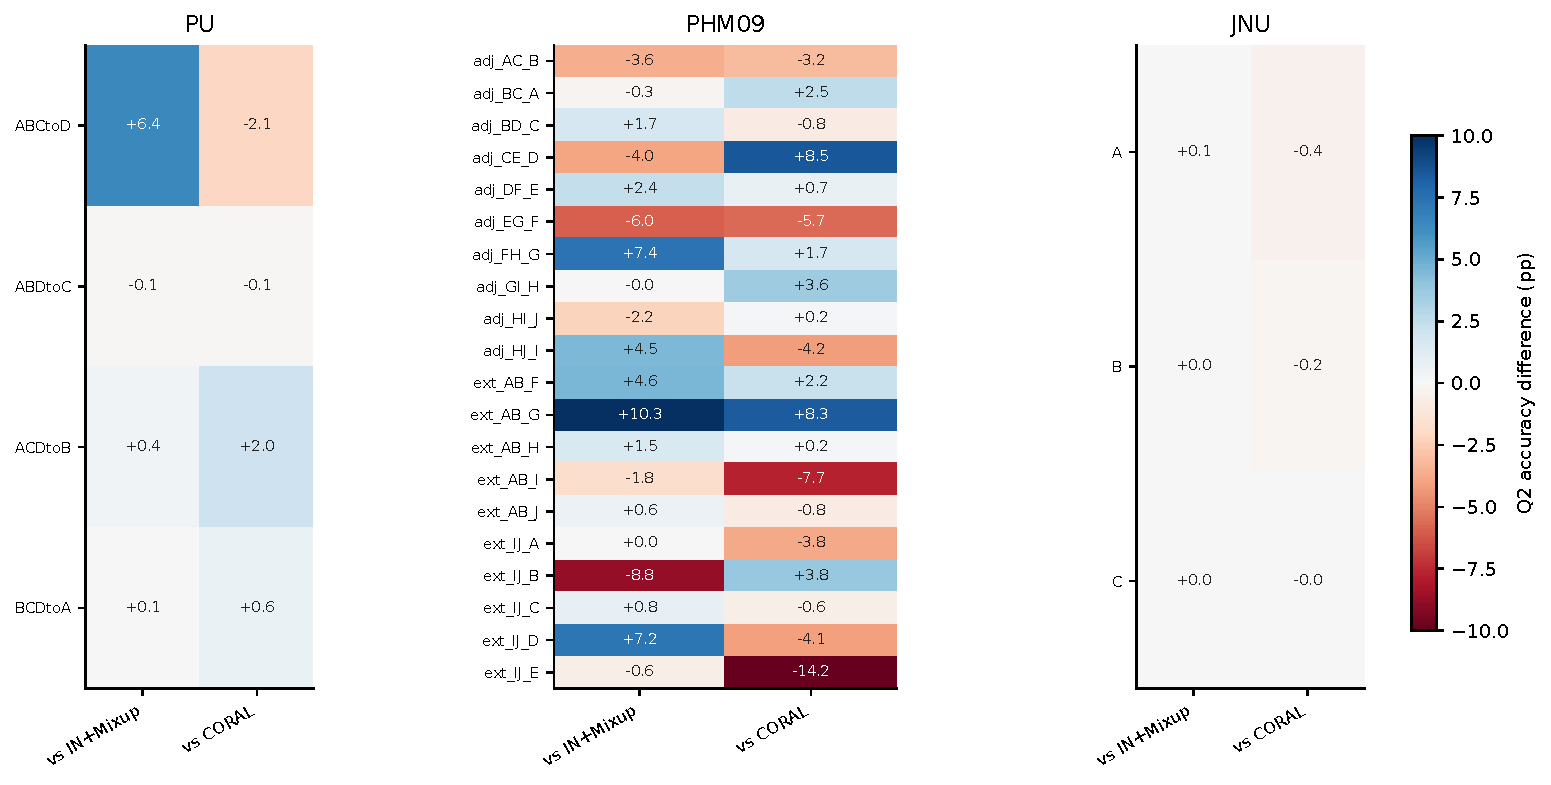
\includegraphics[width=.97\linewidth]{task_differences.pdf}
\caption{Ten-run mean window-accuracy differences on every multi-source task. Blue denotes a Q2 gain and red a loss. The color scale is clipped at $\pm10$ points; cell annotations retain the actual values. All tasks are shown, including unfavorable target conditions.}
\label{fig:task-differences}
\end{figure}
Figure~\ref{fig:task-differences} locates the aggregate changes. On PU, the largest benefit occurs when the target is condition D, at 900 rpm: Q2 improves over matched IN+Mixup from 38.43\% to 44.84\%. The other three targets are already above 91\%, and their changes are much smaller. Deep CORAL remains stronger on D at 46.93\%. Q2's PU advantage is consequently concentrated in a difficult speed-transfer task, together with smaller gains on two other targets.

PHM09 contains both favorable and unfavorable transfers. Q2 gains 10.33 points over matched IN+Mixup on AB$\to$G and 7.24 points on IJ$\to$D, but loses 8.83 points on IJ$\to$B. Gains therefore do not follow only from the number of source conditions or from calling a task extrapolative. The full task table in Appendix~\ref{app:taskresults} retains these differences. The three JNU multi-source tasks have little remaining headroom; their single-source counterparts provide a more demanding extension without redefining the main protocol.

\subsection{What contributes to the event editor?}
\begin{table}[pos=htbp]
\centering\small
\caption{Matched operator ablations: window accuracy (\%), ten runs, fixed final state.}
\label{tab:ablation}
\begin{tabular}{lrrr}
\toprule
Source construction & PU & PHM09 & JNU\\
\midrule
Matched IN+Mixup & $81.44\pm0.98$ & $71.30\pm1.85$ & $99.64\pm0.08$\\
Unedited bank & $81.47\pm1.09$ & $71.29\pm1.90$ & $99.64\pm0.13$\\
Timing, endpoint rates & $82.82\pm1.02$ & $71.59\pm1.16$ & $99.62\pm0.19$\\
Timing, Q2 rates & $82.84\pm0.85$ & $71.26\pm0.84$ & $99.63\pm0.13$\\
Impulse strength only & $81.46\pm1.19$ & $72.58\pm1.52$ & $99.66\pm0.12$\\
Global moment matching & $81.36\pm0.87$ & $71.69\pm1.27$ & $99.69\pm0.07$\\
Proposed Q2 & $83.12\pm0.94$ & $71.98\pm0.95$ & $99.67\pm0.17$\\
\bottomrule
\end{tabular}
\end{table}

Table~\ref{tab:ablation} distinguishes bank sampling from editing and separates the two intervention components. The unedited bank gives 81.47\% on PU and 71.29\% on PHM09, close to matched IN+Mixup. Q2 improves these means to 83.12\% and 71.98\%. Consequently, drawing auxiliary queries from a prepared source bank does not by itself account for the observed increment.

At the same Q2 rates, timing-only editing gives 82.84\%, 71.26\% and 99.63\%. Adding the effective-impulse rule increases dataset-equal accuracy by 0.346 points, with a positive difference in all ten runs. Conversely, adding timing to impulse-only editing increases the dataset-equal mean by 0.355 points, although impulse-only editing is stronger on PHM09. The whole-query moment control matches the edited query's mean and centered RMS, yet remains 0.676 points below Q2 in the dataset-equal summary. The useful change is therefore not fully explained by a global amplitude adjustment.

The two intervention components are not uniformly synergistic. The accuracy interaction $S_Q-S_T-S_A+S_F$ is +0.280 points on PU, $-0.569$ on PHM09 and +0.020 on JNU. The combined construction is beneficial in the main aggregate, but these interactions do not establish a positive coupling effect on every dataset. The endpoint timing recipe is also competitive: its dataset-equal mean is only 0.247 points below Q2. The evidence favors the specified local event construction over the matched simple recipe, rather than an unrestricted claim that stronger event changes always improve diagnosis.

\subsection{Repeatability and checkpoint policy}
\begin{table}[pos=htbp]
\centering\small
\caption{Run-to-run dispersion of window accuracy (percentage points). The dataset statistic is the SD of ten task-averaged scores; within-task SD is averaged over tasks.}
\label{tab:stability}
\begin{tabular}{lrrrrr}
\toprule
Dataset & \multicolumn{2}{c}{Dataset SD} & \multicolumn{2}{c}{Mean within-task SD} & Lower-SD tasks\\
 & IN+Mixup & Q2 & IN+Mixup & Q2 & Q2 / total\\
\midrule
PU & 0.976 & 0.943 & 1.572 & 1.403 & 3/4\\
PHM09 & 1.848 & 0.950 & 5.234 & 4.669 & 13/20\\
JNU & 0.079 & 0.167 & 0.144 & 0.208 & 1/3\\
\bottomrule
\end{tabular}
\end{table}

\begin{figure}[pos=htbp]
\centering
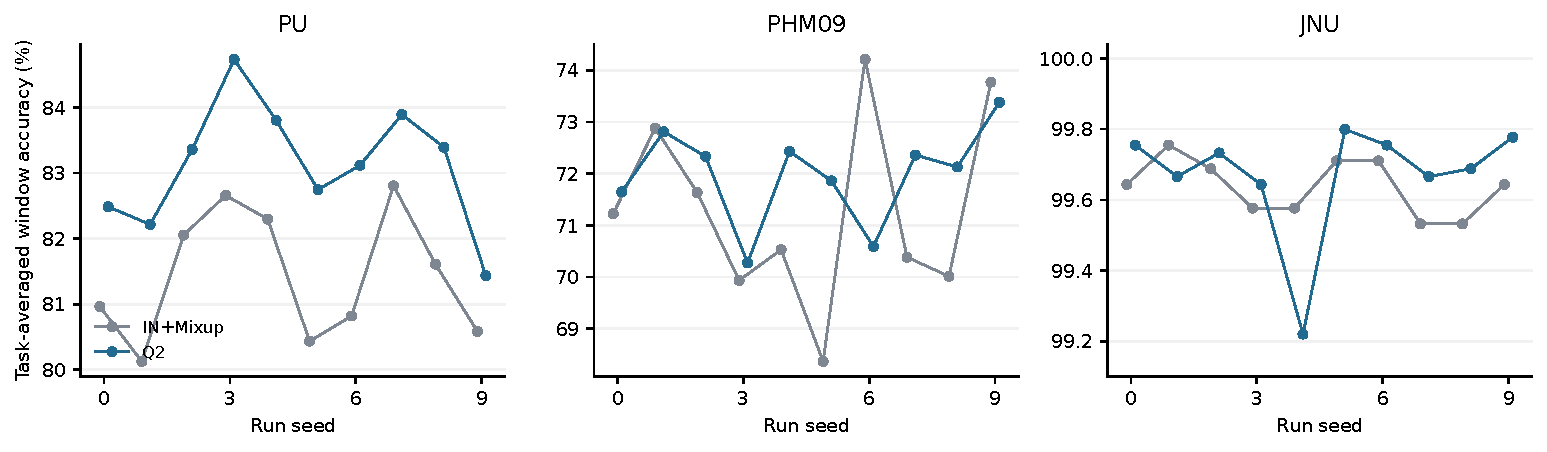
\includegraphics[width=.99\linewidth]{run_stability.pdf}
\caption{Dataset scores for all ten runs under the fixed-final-state policy. Each point first averages the tasks within its dataset. The vertical scales differ to resolve variation near the JNU ceiling.}
\label{fig:stability}
\end{figure}
The PHM09 improvement is accompanied by lower run-to-run dispersion. Its dataset-level accuracy SD falls from 1.848 to 0.950 points, a 48.6\% reduction. The average within-task SD also decreases, from 5.234 to 4.669 points, and 13 of 20 tasks show a reduction. This agreement between aggregate and task-wise summaries supports improved repeatability on PHM09. PU exhibits a smaller aggregate reduction, from 0.976 to 0.943 points, with lower SD on three of four tasks. JNU does not show this pattern: its aggregate SD rises from 0.079 to 0.167 points. Repeatability is therefore a dataset-dependent benefit, not a general noise-robustness claim.

\begin{table}[pos=htbp]
\centering\small
\caption{Source-validation-selected window accuracy (\%) over ten runs. This is a secondary checkpoint policy.}
\label{tab:selection}
\begin{tabular}{lrrr}
\toprule
Method & PU & PHM09 & JNU\\
\midrule
Deep CORAL & $83.04\pm1.04$ & $71.97\pm1.14$ & $99.88\pm0.06$\\
Matched IN+Mixup & $81.38\pm0.92$ & $71.40\pm1.50$ & $99.72\pm0.12$\\
Unedited bank & $81.49\pm1.16$ & $71.39\pm1.46$ & $99.71\pm0.11$\\
Timing, endpoint rates & $82.68\pm1.01$ & $71.79\pm1.07$ & $99.70\pm0.10$\\
Timing, Q2 rates & $82.82\pm0.86$ & $70.92\pm0.93$ & $99.69\pm0.12$\\
Impulse strength only & $81.53\pm1.08$ & $72.95\pm0.92$ & $99.69\pm0.09$\\
Global moment matching & $81.59\pm1.35$ & $73.00\pm1.55$ & $99.75\pm0.09$\\
Proposed Q2 & $83.00\pm1.05$ & $71.58\pm1.22$ & $99.74\pm0.06$\\
\bottomrule
\end{tabular}
\end{table}

Table~\ref{tab:selection} evaluates the source-selected policy on the same trained trajectories. Q2 gives 83.00\%, 71.58\% and 99.74\%, and its dataset-equal advantage over matched IN+Mixup is 0.61 points. This is positive in eight of ten runs. On PHM09, the global-moment control reaches 73.00\% and Deep CORAL reaches 71.97\%, both above Q2. The primary and secondary policies therefore support related but distinct conclusions; the best target outcome is not used to choose between them.

\begin{figure}[pos=htbp]
\centering
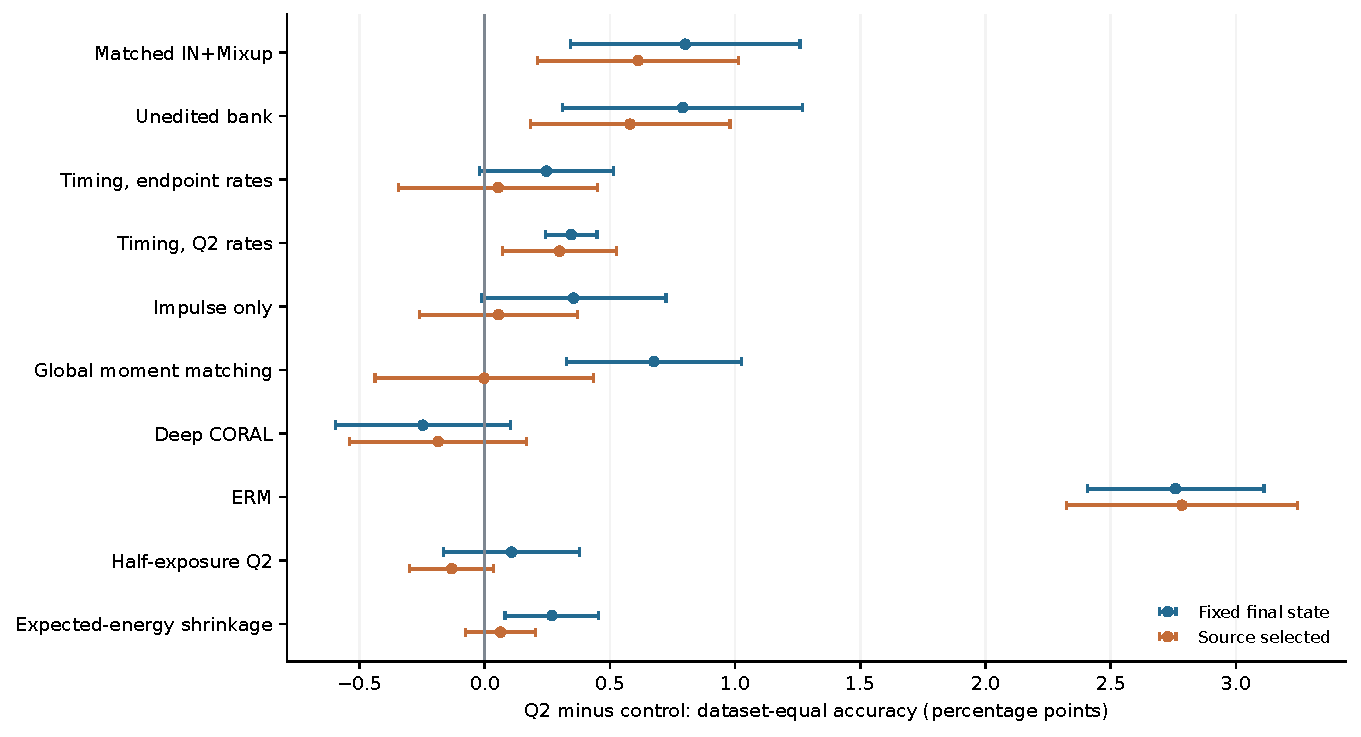
\includegraphics[width=.94\linewidth]{paired_contrasts.pdf}
\caption{Paired dataset-equal accuracy differences under both checkpoint policies. Bars are descriptive 95\% $t_9$ intervals over ten paired run averages, without multiple-comparison adjustment. Zero indicates the control mean. These intervals summarize run variation conditional on the fixed task panel.}
\label{fig:paired}
\end{figure}
Figure~\ref{fig:paired} gives the paired uncertainty summaries. For the primary policy, the Q2-minus-IN+Mixup interval is $[0.342,1.259]$ points; the same-rate timing-only comparison is $[0.243,0.448]$. The comparison with Deep CORAL is $[-0.597,0.103]$. These descriptive results complement, rather than replace, the dataset and task tables. Complete paired values are reported in Appendix~\ref{app:complete}.

\subsection{Recording-level diagnostic errors}
\begin{table}[pos=htbp]
\centering\small
\caption{PU recording-level error rates (\%), ten runs. A lower value is better.}
\label{tab:errors}
\begin{tabular}{lrrr}
\toprule
Method & Healthy false alarms & Faults called healthy & Inner/outer confusion\\
\midrule
Matched IN+Mixup & $3.69\pm2.37$ & $10.41\pm1.79$ & $7.88\pm0.84$\\
Unedited bank & $3.69\pm2.25$ & $10.38\pm1.38$ & $7.41\pm0.88$\\
Proposed Q2 & $3.19\pm1.52$ & $9.12\pm1.06$ & $7.57\pm0.71$\\
Deep CORAL (source domains) & $6.62\pm4.78$ & $8.43\pm1.65$ & $7.97\pm1.72$\\
\bottomrule
\end{tabular}
\par\medskip\begin{minipage}{.98\linewidth}\footnotesize Healthy false alarms use healthy recordings as denominator. The other two rates use all faulty recordings. Scores are computed per task and then averaged within each run; they are empirical classification errors, not system failure probabilities.\end{minipage}
\end{table}

Table~\ref{tab:errors} translates the PU classification results into two practically different errors. Relative to matched IN+Mixup, the fraction of faulty recordings called healthy decreases from 10.41\% to 9.12\%, while healthy false alarms decrease from 3.69\% to 3.19\%. Confusion between inner- and outer-race faults changes from 7.88\% to 7.57\%. These are ten-run, task-averaged recording rates calculated from the saved confusion matrices. They show an improvement in fault recognition without an accompanying increase in the mean false-alarm rate.

Deep CORAL has a lower fault-to-healthy miss rate of 8.43\%, but a higher healthy false-alarm rate of 6.63\%. Q2 and Deep CORAL therefore make different diagnostic trade-offs. No operating threshold is tuned on target data, and the reported errors use the original maximum-probability decisions. The measurements concern classification performance and are not estimates of machine failure probability or maintenance cost.

\subsection{Comparison with physics-guided counterfactual learning}
\begin{table}[pos=htbp]
\centering\footnotesize
\caption{PU recording-level comparison, ten runs, fixed final state. All scores are percentages.}
\label{tab:pcr-last}
\begin{tabular}{lrrr}
\toprule
Recipe & Accuracy & Macro-F1 & Balanced accuracy\\
\midrule
Q2, short vibration input & $84.81\pm1.04$ & $84.00\pm1.08$ & $87.81\pm0.83$\\
Matched IN+Mixup & $83.33\pm1.39$ & $82.74\pm1.49$ & $86.58\pm1.24$\\
Unedited bank & $83.78\pm1.24$ & $83.03\pm1.15$ & $86.92\pm1.13$\\
Native 40-rev. author CE & $85.58\pm1.65$ & $82.07\pm1.37$ & $84.59\pm1.96$\\
Native 40-rev. CE+real healthy & $85.32\pm1.95$ & $82.35\pm1.72$ & $85.68\pm2.06$\\
Native 40-rev. PCR & $82.51\pm0.64$ & $80.28\pm0.97$ & $84.37\pm1.09$\\
Short-input author CE & $84.30\pm0.84$ & $76.39\pm0.67$ & $75.79\pm0.94$\\
Short-input CE+real healthy & $84.09\pm0.93$ & $76.10\pm0.93$ & $75.91\pm0.94$\\
Short-input PCR & $83.99\pm0.98$ & $75.95\pm1.14$ & $74.99\pm1.61$\\
\bottomrule
\end{tabular}
\par\medskip\begin{minipage}{.98\linewidth}\footnotesize Native PCR uses recorded speed to construct 40-revolution inputs. The comparison aligns recording roles, not input windows or architectures. This is a declared cross-condition adaptation of a single-source cross-machine method.\end{minipage}
\end{table}

Table~\ref{tab:pcr-last} compares Q2 with the implemented PCR-OIPN variants \cite{pcr2026}. Their native 40-revolution inputs cover different windows from the short-input models. Predictions are therefore compared after averaging probabilities over the same PU recording roles. Q2 gives 84.81\% recording accuracy, 84.00\% macro-F1 and 87.81\% BA, compared with 82.51\%, 80.28\% and 84.37\% for native PCR. The native author CE baseline attains higher recording accuracy at 85.58\%, but lower macro-F1 and BA. The comparison does not imply that all benefits arise from counterfactual learning or that Q2 dominates all evaluation metrics.

The information requirements also differ. The native angular frontend uses recorded target speed to form the 40-revolution input; Q2's deployed frontend uses vibration alone. All variants retain their declared frontends and training rules. This experiment evaluates a multi-source cross-condition adaptation, whereas the original PCR study addresses single-source cross-machine diagnosis. It is included as a mechanism-related comparison, without substituting published results obtained under a different protocol.

\subsection{Reduced source coverage on JNU}
\begin{table}[pos=htbp]
\centering\small
\caption{JNU single-source extension: all six source--target directions, ten runs.}
\label{tab:sdg}
\begin{tabular}{llrrr}
\toprule
Policy & Method & Accuracy & Macro-F1 & Recording BA\\
\midrule
Final & IN+Mixup & $94.95\pm1.05$ & $94.72\pm0.90$ & $99.17\pm1.76$\\
Final & Unedited bank & $95.61\pm0.72$ & $95.32\pm0.65$ & $99.58\pm1.32$\\
Final & Q2 & $95.72\pm0.74$ & $95.44\pm0.63$ & $99.17\pm1.76$\\
Source-selected & IN+Mixup & $95.28\pm0.90$ & $94.89\pm0.74$ & $97.92\pm2.20$\\
Source-selected & Unedited bank & $94.78\pm1.54$ & $94.52\pm1.25$ & $98.33\pm2.15$\\
Source-selected & Q2 & $95.22\pm1.11$ & $94.85\pm0.91$ & $98.75\pm2.01$\\
\bottomrule
\end{tabular}
\end{table}

The single-source extension trains from one JNU speed and evaluates on each of the other two, yielding six directions. Source event analysis uses two legal training contexts from the same source speed; it does not introduce an additional observed condition. Each of the three methods trains three source models per run, and each frozen model supplies two target evaluations.

The fixed-final-state accuracy decreases from the near-ceiling multi-source values to 94.95\% for IN+Mixup, 95.61\% for the unedited bank and 95.72\% for Q2 (Table~\ref{tab:sdg}). The 0.77-point Q2 increment over IN+Mixup is mostly accompanied by the change to bank sampling: the increment over the unedited bank is only 0.11 points. Under source selection, Q2 is also slightly below IN+Mixup. These results demonstrate that the operator remains usable with a source-local analyzer, while providing limited evidence for a distinct single-source editing advantage. The six directions are all retained in the appendix.

\subsection{Editing measured source signals}
Figure~\ref{fig:source-edit} shows actual source queries and their event edits.
Selection uses metadata alone: for each dataset, take the first task in lexical
order at seed 0, class 1, the first source-domain/record identifier, and the
middle of its three registered query locations. The corresponding class-0
examples and identifiers are provided in Appendix~\ref{app:source-examples}.
All event coefficients and source contexts are reused from the frozen source
bank construction. No target predictions determine these selections.

\begin{figure}[pos=htbp]
\centering
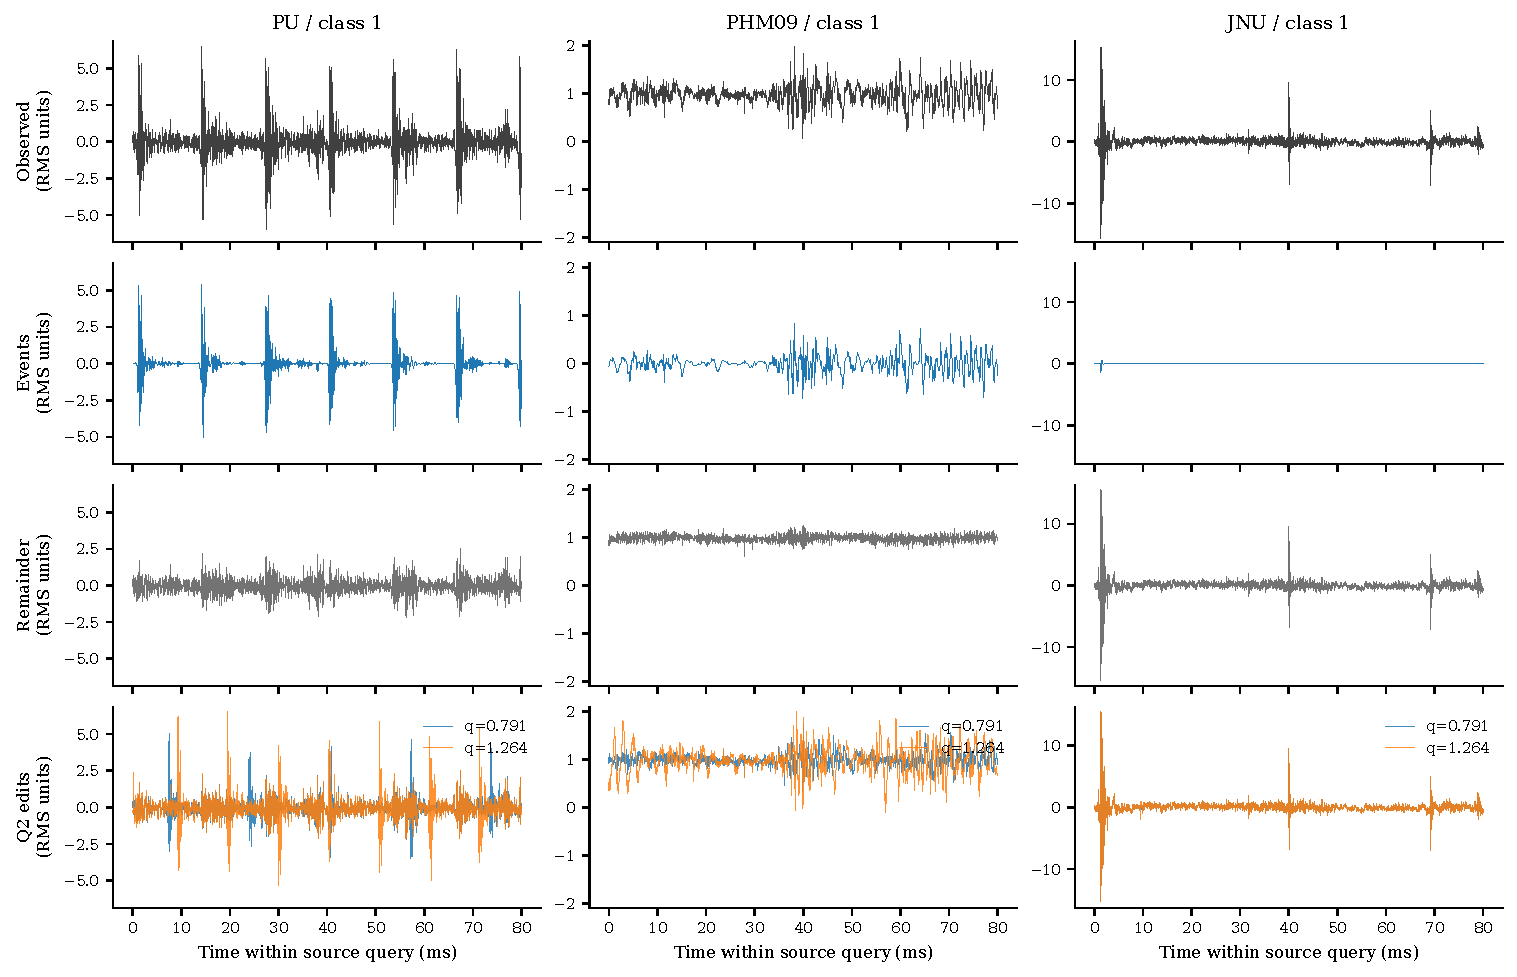
\includegraphics[width=.99\linewidth]{generated/real_source_edits.pdf}
\caption{Measured-source examples selected by the fixed metadata rule. Rows show
the observed query, estimated event component, retained remainder and two Q2
edits. Columns correspond to PU outer-race class, PHM09 configuration 2 and JNU
inner-race class. Time covers the entire registered query; all four rows in a
column share the same amplitude scale, divided by that observed query's RMS.
The weak estimated event in the selected JNU query is retained in the figure.}
\label{fig:source-edit}
\end{figure}

The examples show that the editor adapts its effective action to the estimated
event component. In the selected PU query, clear repeated transients enter the
event component and their locations change. The PHM09 example also retains a
substantial observation term. In the JNU example, most observed structure
remains in the remainder, so the edit is weak on this query. Neither the event
energy nor the remainder energy is interpreted as a separately measured
physical-factor share. Classification utility is assessed by the matched
experiments rather than by visually selecting a clean decomposition.


\section{Discussion}
\subsection{Interpretation of the mechanism}
The proposed editor makes an explicit distinction between event occurrence, effective impulse strength, response shape and the retained observation. Its intervention has a defined action before the diagnostic representation is learned. The unit-rate identity and fixed-response construction establish properties of the operator, while the matched ablations establish its empirical diagnostic contribution. Reconstruction quality alone would not establish either label preservation or improved transfer.

This interpretation also clarifies the role of the other components. IN and Mixup are effective parts of the classifier recipe, and the log-spectrum frontend supplies a compact frequency representation. The matched comparisons keep these components fixed, so the remaining Q2 increment can be attributed to the specified source construction within that recipe. They do not show that the event editor is the largest contributor to the complete system or that it is indispensable on every dataset. The PHM09 alignment baseline and impulse-only control provide substantive alternative explanations for parts of the performance.

The event model specifies a local, model-based intervention. Its estimated coefficients are not direct physical measurements of every impact, and the remainder can contain both fault information and condition effects. The fixed strength--rate coupling is an augmentation rule, not a universal load--speed law. Because the remainder retains its observed coordinates, the edit is narrower than a complete physical change of shaft speed. This selective construction avoids deleting unexplained fault evidence while creating controlled variation in a plausible signal-generation mechanism.

\subsection{Deployment and computational implications}
The event analyzer and source bank are used only during preparation and training. Q2 and its matched IN+Mixup control have identical deployed networks: 2,200,627 parameters on PU, 2,201,272 on PHM09 and 2,200,756 on JNU. Convolution and linear layers require approximately 5.751 million multiply--accumulates per window, excluding the FFT frontend, normalization, activations and memory operations. Thus the editor adds no deployed trainable parameters or convolution/linear operations.

Source preparation has a real cost. A previously audited three-run preparation campaign built 81 task/run banks from 3372 context groups in 52.69 minutes, including all five rendered rates, control features, I/O and fingerprint checks. This measurement reuses existing 500-iteration numerical fits and is neither the initial inverse-fitting time nor the total ten-run cost. The matched classification arms share 2000 updates and the same batch layout. The practical benefit is therefore a separation between offline source construction and ordinary online diagnosis, rather than a claim of cost-free augmentation.

\subsection{Application scope}
The experiments evaluate transfer across recorded conditions. PU repeats bearing identities across conditions; PHM09 configuration labels do not identify gearbox serial units; JNU uses separated time blocks of existing recordings. The three datasets therefore support cross-condition diagnosis under the stated protocols, with the multi-source and single-source settings kept distinct. Cross-machine confirmation would require a corresponding evaluation design.

The current evidence is strongest for a selective source intervention that improves a fixed, strong classifier recipe on PU and PHM09. It also shows more repeatable PHM09 training and lower PU recording-level error rates. Deep CORAL remains a strong competitor, source selection changes some rankings, and JNU offers limited multi-source headroom. Future work can examine event-model adequacy and intervention-strength selection using source evidence, together with testing under explicitly measured disturbance and machine changes. Those extensions are separate from the completed experiments reported here.

\section{Conclusion}
This paper proposes observation-anchored event-mechanism editing for fault diagnosis under unseen operating conditions. A source-only sparse analyzer supplies events and response kernels; the editor changes event timing and effective impulse strength while preserving the remainder of each measured observation. The resulting source views train a conventional classifier with vibration-only deployment.

Across 27 multi-source tasks and ten runs, Q2 improves dataset-equal accuracy by 0.80 percentage points over matched IN+Mixup and by 0.79 points over an unedited-bank control. Timing-only and moment-matched comparisons support a contribution from the specified event construction. The method also reduces PU recording-level missed faults and improves PHM09 repeatability. Strong alignment baselines and the single-source extension show that these benefits are condition-dependent. The results establish observation-anchored event editing as a practical source-training mechanism whose diagnostic contribution can be measured without adding complexity to the deployed model.

\appendix
\FloatBarrier
\section{Task inventory and implementation details}
\label{app:tasks}
PU uses BCD$\to$A, ACD$\to$B, ABD$\to$C and ABC$\to$D. JNU uses
BC$\to$A, AC$\to$B and AB$\to$C. PHM09 adjacent-domain tasks are
AC$\to$B, BC$\to$A, BD$\to$C, CE$\to$D, DF$\to$E,
EG$\to$F, FH$\to$G, GI$\to$H, HI$\to$J and HJ$\to$I.
Its distant-domain tasks are AB$\to$F/G/H/I/J and IJ$\to$A/B/C/D/E,
where each target letter defines a separate task.

Source context length is 32768 samples and response support is 4 ms.
The four carrier candidates per context are selected from source spectra above
four times the largest paired source shaft rate and below 0.44 times the
sampling frequency. Candidate peaks are separated by at least
$\max(100,3f_s/N)$ Hz. Each carrier is combined with decay constants
0.25, 0.5 and 1 ms and phases 0, $\pi/2$, $\pi$ and $3\pi/2$.
The kernel is an exponentially decaying sinusoid multiplied by a squared
cosine taper and normalized by its discrete $\ell_2$ norm.
Numerical coefficients are obtained by the fixed accelerated proximal solver;
the classifier does not update them.
The reused numerical fits use 500 proximal iterations. Their penalties are
specified from each normalized source context. Let
\begin{equation}
 \nu_j=\max\!\left\{
 \frac{\operatorname{median}_{f\in[0.45,0.5]}
       |\operatorname{rFFT}(\bar x_j)[f]|}{\sqrt{N\log 2}},
 0.005\sqrt{\frac1N\sum_t\bar x_j[t]^2}\right\},
\end{equation}
where $f$ is normalized frequency, and define
\begin{equation}
 b(G)=\frac{\nu_1+\nu_2}{2}
 \sqrt{4+4\sqrt{\log(\max(G,2))}+2\log(\max(G,2))}.
\end{equation}
Then $\lambda_{s,j}=\nu_j\sqrt{2\log(2\cdot48N)}$,
$\lambda_b=b(4)$ and $\lambda_c=b(\max(G_F,1))$, where $G_F$ is the number
of stationary frequency candidates. The proximal step uses the fixed
spectral-norm upper bound formed from the convolution, shaft-harmonic and
stationary dictionaries. These numerical settings are source-derived and
are reused for all edited views of a context.

\subsection{Source-domain alignment baselines}
For DANN, a source-domain head maps the shared 256-dimensional representation to 128 hidden units with ReLU and then to source-domain logits. The gradient-reversal coefficient follows $2/(1+\exp(-10p))-1$, where $p$ is training progress, and is applied once. Deep CORAL averages covariance discrepancies between each source pair, using unbiased sample covariance and squared Frobenius distance divided by $4d^2$, where $d=256$. Its alignment weight is one. Both baselines retain the same source pools and fixed training schedule as the ERM baseline. They do not perform target adaptation.

\subsection{Exposure controls}
Conditional on the original edit mask, half exposure retains an edit with probability 0.5 and otherwise uses the same clean bank query. The expected edited fraction of auxiliary positions falls from 0.5 to 0.25. The expected-energy control instead scales every log-feature edit difference by $\sqrt{0.5}$. All other training choices are unchanged.
\begin{table}[pos=htbp]
\centering\small
\caption{Exposure controls: window accuracy (\%) over ten runs at the fixed final state.}
\label{tab:exposure}
\begin{tabular}{lrrr}
\toprule
Method & PU & PHM09 & JNU\\
\midrule
Expected-energy shrinkage & $82.51\pm1.17$ & $71.81\pm1.24$ & $99.65\pm0.12$\\
Half-exposure Q2 & $82.82\pm1.06$ & $71.94\pm1.13$ & $99.69\pm0.08$\\
Standard Q2 & $83.12\pm0.94$ & $71.98\pm0.95$ & $99.67\pm0.17$\\
\bottomrule
\end{tabular}
\end{table}

Standard Q2 exceeds half exposure by 0.107 points in the primary dataset-equal mean, with only five of ten paired differences positive. Under source selection, half exposure is 0.132 points higher. This sensitivity does not justify replacing the fixed main recipe; both policies and all exposure rows are retained.

\FloatBarrier
\section{Complete comparison and paired summaries}
\label{app:complete}
The following tables retain all 22 multi-source recipes. The main comparisons use the fixed final state; source selection is reported separately. The poor MOCD equation-literal result is kept as an implementation-interpretation result and is not used to characterize the original method's published performance. Each table reports ten-run mean$\pm$sample SD with the task weighting in Eq.~\eqref{eq:aggregation}.
\begin{table}[pos=htbp]
\centering\footnotesize
\caption{Fixed-final-state window accuracy (\%) for all 22 complete recipes, ten runs.}
\label{tab:all-last}
\begin{tabular}{lrrr}
\toprule
Recipe & PU & PHM09 & JNU\\
\midrule
Author-backbone CE & $80.63\pm1.38$ & $51.37\pm1.93$ & $83.95\pm7.88$\\
Author-backbone IN+Mixup & $81.85\pm0.85$ & $68.23\pm1.06$ & $95.31\pm4.86$\\
Archived identity+Mixup & $80.86\pm0.39$ & $67.68\pm1.40$ & $99.68\pm0.26$\\
Archived IN+Mixup & $81.35\pm0.94$ & $71.35\pm1.39$ & $99.59\pm0.14$\\
CCDG (author feature core) & $81.13\pm1.16$ & $57.47\pm1.73$ & $87.19\pm8.11$\\
Earlier event editor & $82.59\pm0.97$ & $71.46\pm1.35$ & $99.55\pm0.17$\\
MOCD (literal equation) & $80.66\pm1.76$ & $10.31\pm1.47$ & $29.66\pm24.80$\\
MOCD (prose interpretation) & $80.50\pm0.93$ & $65.26\pm2.51$ & $95.14\pm2.86$\\
Whole-waveform scaling & $80.63\pm1.29$ & $68.34\pm1.02$ & $99.11\pm0.30$\\
Archived intact control & $81.13\pm0.82$ & $71.60\pm1.44$ & $99.60\pm0.21$\\
DANN (source domains) & $80.81\pm1.52$ & $52.94\pm2.40$ & $82.47\pm10.02$\\
Deep CORAL (source domains) & $82.99\pm1.14$ & $72.65\pm1.25$ & $99.87\pm0.06$\\
ERM (shared CNN+IN) & $82.97\pm1.34$ & $63.81\pm0.99$ & $99.71\pm0.14$\\
Impulse strength only & $81.46\pm1.19$ & $72.58\pm1.52$ & $99.66\pm0.12$\\
Matched IN+Mixup & $81.44\pm0.98$ & $71.30\pm1.85$ & $99.64\pm0.08$\\
Timing, endpoint rates & $82.82\pm1.02$ & $71.59\pm1.16$ & $99.62\pm0.19$\\
Unedited bank & $81.47\pm1.09$ & $71.29\pm1.90$ & $99.64\pm0.13$\\
Global moment matching & $81.36\pm0.87$ & $71.69\pm1.27$ & $99.69\pm0.07$\\
Proposed Q2 & $83.12\pm0.94$ & $71.98\pm0.95$ & $99.67\pm0.17$\\
Timing, Q2 rates & $82.84\pm0.85$ & $71.26\pm0.84$ & $99.63\pm0.13$\\
Expected-energy shrinkage & $82.51\pm1.17$ & $71.81\pm1.24$ & $99.65\pm0.12$\\
Half-exposure Q2 & $82.82\pm1.06$ & $71.94\pm1.13$ & $99.69\pm0.08$\\
\bottomrule
\end{tabular}
\end{table}

\begin{table}[pos=htbp]
\centering\footnotesize
\caption{Source-selected window accuracy (\%) for all 22 complete recipes, ten runs.}
\label{tab:all-selected}
\begin{tabular}{lrrr}
\toprule
Recipe & PU & PHM09 & JNU\\
\midrule
Author-backbone CE & $80.63\pm1.38$ & $50.97\pm2.17$ & $83.94\pm7.42$\\
Author-backbone IN+Mixup & $81.85\pm0.85$ & $65.20\pm1.40$ & $95.03\pm5.11$\\
Archived identity+Mixup & $80.89\pm0.36$ & $67.05\pm2.00$ & $99.04\pm1.04$\\
Archived IN+Mixup & $81.42\pm0.91$ & $71.82\pm1.52$ & $99.69\pm0.17$\\
CCDG (author feature core) & $81.13\pm1.16$ & $55.76\pm1.26$ & $86.71\pm8.00$\\
Earlier event editor & $82.58\pm0.99$ & $71.57\pm1.37$ & $99.69\pm0.17$\\
MOCD (literal equation) & $80.80\pm1.56$ & $11.82\pm0.79$ & $53.50\pm28.66$\\
MOCD (prose interpretation) & $80.52\pm1.36$ & $60.79\pm3.54$ & $95.70\pm4.06$\\
Whole-waveform scaling & $81.21\pm1.17$ & $67.48\pm0.84$ & $99.25\pm0.30$\\
Archived intact control & $81.15\pm0.78$ & $71.68\pm1.19$ & $99.71\pm0.11$\\
DANN (source domains) & $80.85\pm2.27$ & $52.49\pm2.30$ & $79.41\pm9.55$\\
Deep CORAL (source domains) & $83.04\pm1.04$ & $71.97\pm1.14$ & $99.88\pm0.06$\\
ERM (shared CNN+IN) & $82.95\pm1.02$ & $63.35\pm0.93$ & $99.67\pm0.16$\\
Impulse strength only & $81.53\pm1.08$ & $72.95\pm0.92$ & $99.69\pm0.09$\\
Matched IN+Mixup & $81.38\pm0.92$ & $71.40\pm1.50$ & $99.72\pm0.12$\\
Timing, endpoint rates & $82.68\pm1.01$ & $71.79\pm1.07$ & $99.70\pm0.10$\\
Unedited bank & $81.49\pm1.16$ & $71.39\pm1.46$ & $99.71\pm0.11$\\
Global moment matching & $81.59\pm1.35$ & $73.00\pm1.55$ & $99.75\pm0.09$\\
Proposed Q2 & $83.00\pm1.05$ & $71.58\pm1.22$ & $99.74\pm0.06$\\
Timing, Q2 rates & $82.82\pm0.86$ & $70.92\pm0.93$ & $99.69\pm0.12$\\
Expected-energy shrinkage & $82.49\pm1.37$ & $71.97\pm1.49$ & $99.68\pm0.10$\\
Half-exposure Q2 & $82.84\pm1.27$ & $72.18\pm1.17$ & $99.71\pm0.07$\\
\bottomrule
\end{tabular}
\end{table}

\begin{table}[pos=htbp]
\centering\small
\caption{Dataset-equal paired accuracy differences: Q2 minus each control (percentage points). Intervals are descriptive 95\% $t_9$ intervals over ten paired run averages.}
\label{tab:paired}
\begin{tabular}{lrrr}
\toprule
Control & Mean difference & 95\% interval & Positive runs\\
\midrule
Matched IN+Mixup & $+0.801$ & $[+0.342, +1.259]$ & 9/10\\
Unedited bank & $+0.791$ & $[+0.312, +1.270]$ & 9/10\\
Timing, endpoint rates & $+0.247$ & $[-0.021, +0.514]$ & 7/10\\
Timing, Q2 rates & $+0.346$ & $[+0.243, +0.448]$ & 10/10\\
Impulse only & $+0.355$ & $[-0.013, +0.724]$ & 9/10\\
Global moment matching & $+0.676$ & $[+0.325, +1.027]$ & 9/10\\
Half-exposure Q2 & $+0.107$ & $[-0.163, +0.378]$ & 5/10\\
Expected-energy shrinkage & $+0.268$ & $[+0.081, +0.456]$ & 9/10\\
Deep CORAL & $-0.247$ & $[-0.597, +0.103]$ & 3/10\\
ERM & $+2.759$ & $[+2.406, +3.112]$ & 10/10\\
\bottomrule
\end{tabular}
\par\medskip\begin{minipage}{.98\linewidth}\footnotesize These post-result intervals are unadjusted for multiple comparisons and conditional on the fixed task panel; they are not intervals over independent machine populations.\end{minipage}
\end{table}

\begin{table}[pos=htbp]
\centering\footnotesize
\caption{Fixed-final-state window macro-F1 (\%) for all 22 recipes, ten runs.}
\label{tab:all-last-macro_f1}
\begin{tabular}{lrrr}
\toprule
Recipe & PU & PHM09 & JNU\\
\midrule
Author-backbone CE & $78.68\pm1.18$ & $44.91\pm2.13$ & $85.24\pm6.36$\\
Author-backbone IN+Mixup & $80.32\pm0.86$ & $64.50\pm1.49$ & $96.14\pm3.66$\\
Archived identity+Mixup & $79.81\pm0.49$ & $63.98\pm1.43$ & $99.67\pm0.26$\\
Archived IN+Mixup & $79.92\pm0.90$ & $67.85\pm1.76$ & $99.57\pm0.15$\\
CCDG (author feature core) & $79.11\pm1.10$ & $52.04\pm1.86$ & $89.29\pm6.70$\\
Earlier event editor & $81.01\pm0.93$ & $68.36\pm1.29$ & $99.53\pm0.18$\\
MOCD (literal equation) & $78.11\pm1.78$ & $3.56\pm0.66$ & $26.02\pm23.92$\\
MOCD (prose interpretation) & $77.90\pm0.94$ & $60.41\pm2.84$ & $94.51\pm2.02$\\
Whole-waveform scaling & $79.03\pm1.24$ & $64.61\pm1.05$ & $99.03\pm0.31$\\
Archived intact control & $79.64\pm0.90$ & $68.17\pm1.82$ & $99.57\pm0.21$\\
DANN (source domains) & $79.54\pm1.31$ & $46.15\pm2.75$ & $79.61\pm9.72$\\
Deep CORAL (source domains) & $81.27\pm1.00$ & $68.69\pm1.44$ & $99.84\pm0.07$\\
ERM (shared CNN+IN) & $81.51\pm1.34$ & $58.51\pm1.21$ & $99.67\pm0.17$\\
Impulse strength only & $80.03\pm1.09$ & $69.63\pm1.63$ & $99.64\pm0.12$\\
Matched IN+Mixup & $80.07\pm1.02$ & $67.75\pm2.15$ & $99.62\pm0.09$\\
Timing, endpoint rates & $81.23\pm0.87$ & $68.43\pm1.06$ & $99.60\pm0.21$\\
Unedited bank & $80.00\pm0.96$ & $67.81\pm2.06$ & $99.63\pm0.13$\\
Global moment matching & $79.39\pm0.69$ & $68.59\pm1.38$ & $99.68\pm0.07$\\
Proposed Q2 & $81.57\pm0.85$ & $68.66\pm1.18$ & $99.65\pm0.17$\\
Timing, Q2 rates & $81.33\pm0.75$ & $67.87\pm0.95$ & $99.61\pm0.14$\\
Expected-energy shrinkage & $80.97\pm1.02$ & $68.61\pm1.35$ & $99.62\pm0.11$\\
Half-exposure Q2 & $81.32\pm0.97$ & $68.74\pm1.33$ & $99.67\pm0.09$\\
\bottomrule
\end{tabular}
\end{table}

\begin{table}[pos=htbp]
\centering\footnotesize
\caption{Source-selected window macro-F1 (\%) for all 22 recipes, ten runs.}
\label{tab:all-selected-macro_f1}
\begin{tabular}{lrrr}
\toprule
Recipe & PU & PHM09 & JNU\\
\midrule
Author-backbone CE & $78.68\pm1.18$ & $44.45\pm2.46$ & $84.73\pm5.80$\\
Author-backbone IN+Mixup & $80.32\pm0.86$ & $61.21\pm1.66$ & $95.73\pm3.77$\\
Archived identity+Mixup & $79.83\pm0.42$ & $63.43\pm1.98$ & $99.05\pm0.98$\\
Archived IN+Mixup & $79.94\pm0.79$ & $68.09\pm1.77$ & $99.68\pm0.17$\\
CCDG (author feature core) & $79.11\pm1.10$ & $50.04\pm1.30$ & $88.39\pm6.80$\\
Earlier event editor & $81.01\pm0.97$ & $68.28\pm1.36$ & $99.67\pm0.18$\\
MOCD (literal equation) & $78.34\pm1.74$ & $2.82\pm0.29$ & $47.41\pm27.54$\\
MOCD (prose interpretation) & $77.87\pm1.50$ & $55.26\pm4.02$ & $95.59\pm3.10$\\
Whole-waveform scaling & $79.53\pm1.07$ & $63.38\pm0.88$ & $99.20\pm0.31$\\
Archived intact control & $79.68\pm0.85$ & $68.01\pm1.33$ & $99.69\pm0.11$\\
DANN (source domains) & $79.41\pm1.92$ & $45.56\pm2.91$ & $76.58\pm8.47$\\
Deep CORAL (source domains) & $81.32\pm0.81$ & $68.00\pm1.31$ & $99.86\pm0.08$\\
ERM (shared CNN+IN) & $81.39\pm1.04$ & $57.94\pm1.15$ & $99.62\pm0.20$\\
Impulse strength only & $80.07\pm1.04$ & $69.64\pm1.09$ & $99.67\pm0.09$\\
Matched IN+Mixup & $80.01\pm0.97$ & $67.68\pm1.77$ & $99.71\pm0.12$\\
Timing, endpoint rates & $81.11\pm0.82$ & $68.45\pm1.17$ & $99.68\pm0.10$\\
Unedited bank & $79.99\pm1.06$ & $67.64\pm1.60$ & $99.69\pm0.10$\\
Global moment matching & $79.55\pm1.21$ & $69.64\pm1.78$ & $99.74\pm0.09$\\
Proposed Q2 & $81.44\pm0.93$ & $68.06\pm1.54$ & $99.73\pm0.06$\\
Timing, Q2 rates & $81.28\pm0.76$ & $67.24\pm1.24$ & $99.67\pm0.12$\\
Expected-energy shrinkage & $80.92\pm1.23$ & $68.56\pm1.68$ & $99.67\pm0.10$\\
Half-exposure Q2 & $81.31\pm1.18$ & $68.84\pm1.30$ & $99.70\pm0.07$\\
\bottomrule
\end{tabular}
\end{table}

\begin{table}[pos=htbp]
\centering\footnotesize
\caption{Fixed-final-state recording balanced accuracy (\%) for all 22 recipes, ten runs.}
\label{tab:all-last-recording_ba}
\begin{tabular}{lrrr}
\toprule
Recipe & PU & PHM09 & JNU\\
\midrule
Author-backbone CE & $82.47\pm1.54$ & $53.41\pm2.18$ & $92.50\pm4.73$\\
Author-backbone IN+Mixup & $86.70\pm1.02$ & $72.50\pm2.02$ & $98.33\pm3.51$\\
Archived identity+Mixup & $86.20\pm0.87$ & $70.25\pm2.02$ & $100.00\pm0.00$\\
Archived IN+Mixup & $86.57\pm1.47$ & $74.62\pm2.25$ & $100.00\pm0.00$\\
CCDG (author feature core) & $83.53\pm2.15$ & $59.00\pm2.16$ & $94.17\pm4.03$\\
Earlier event editor & $87.42\pm1.01$ & $76.97\pm1.52$ & $100.00\pm0.00$\\
MOCD (literal equation) & $84.84\pm3.23$ & $11.09\pm1.57$ & $30.00\pm25.22$\\
MOCD (prose interpretation) & $86.01\pm1.98$ & $67.72\pm3.46$ & $100.00\pm0.00$\\
Whole-waveform scaling & $86.69\pm1.54$ & $72.88\pm2.20$ & $100.00\pm0.00$\\
Archived intact control & $86.51\pm1.46$ & $75.69\pm2.40$ & $100.00\pm0.00$\\
DANN (source domains) & $87.01\pm1.96$ & $54.44\pm1.71$ & $88.33\pm8.05$\\
Deep CORAL (source domains) & $86.86\pm1.92$ & $75.56\pm1.52$ & $100.00\pm0.00$\\
ERM (shared CNN+IN) & $86.97\pm2.43$ & $66.16\pm1.02$ & $100.00\pm0.00$\\
Impulse strength only & $86.86\pm1.12$ & $77.44\pm2.19$ & $100.00\pm0.00$\\
Matched IN+Mixup & $86.58\pm1.24$ & $74.94\pm2.95$ & $100.00\pm0.00$\\
Timing, endpoint rates & $87.79\pm1.11$ & $76.91\pm1.64$ & $100.00\pm0.00$\\
Unedited bank & $86.92\pm1.13$ & $75.47\pm2.85$ & $100.00\pm0.00$\\
Global moment matching & $87.06\pm0.99$ & $75.97\pm2.15$ & $100.00\pm0.00$\\
Proposed Q2 & $87.81\pm0.83$ & $76.72\pm1.71$ & $100.00\pm0.00$\\
Timing, Q2 rates & $87.71\pm0.79$ & $76.06\pm0.97$ & $100.00\pm0.00$\\
Expected-energy shrinkage & $87.81\pm0.95$ & $75.69\pm1.59$ & $100.00\pm0.00$\\
Half-exposure Q2 & $87.68\pm1.09$ & $75.53\pm1.93$ & $100.00\pm0.00$\\
\bottomrule
\end{tabular}
\end{table}

\begin{table}[pos=htbp]
\centering\footnotesize
\caption{Source-selected recording balanced accuracy (\%) for all 22 recipes, ten runs.}
\label{tab:all-selected-recording_ba}
\begin{tabular}{lrrr}
\toprule
Recipe & PU & PHM09 & JNU\\
\midrule
Author-backbone CE & $82.47\pm1.54$ & $53.25\pm2.16$ & $92.50\pm4.73$\\
Author-backbone IN+Mixup & $86.70\pm1.02$ & $69.19\pm2.30$ & $97.50\pm4.03$\\
Archived identity+Mixup & $86.27\pm0.74$ & $69.16\pm2.64$ & $100.00\pm0.00$\\
Archived IN+Mixup & $86.40\pm1.20$ & $75.22\pm2.13$ & $100.00\pm0.00$\\
CCDG (author feature core) & $83.53\pm2.15$ & $57.72\pm1.74$ & $94.17\pm4.03$\\
Earlier event editor & $87.27\pm1.16$ & $76.47\pm1.65$ & $100.00\pm0.00$\\
MOCD (literal equation) & $84.60\pm3.70$ & $11.88\pm0.92$ & $52.50\pm25.17$\\
MOCD (prose interpretation) & $85.67\pm1.32$ & $62.38\pm4.22$ & $100.00\pm0.00$\\
Whole-waveform scaling & $86.99\pm1.17$ & $71.66\pm1.60$ & $100.00\pm0.00$\\
Archived intact control & $86.46\pm1.59$ & $75.25\pm1.34$ & $100.00\pm0.00$\\
DANN (source domains) & $86.97\pm2.30$ & $53.91\pm2.32$ & $87.50\pm7.08$\\
Deep CORAL (source domains) & $86.77\pm1.66$ & $75.25\pm1.36$ & $100.00\pm0.00$\\
ERM (shared CNN+IN) & $86.73\pm1.63$ & $65.47\pm0.85$ & $100.00\pm0.00$\\
Impulse strength only & $86.88\pm1.12$ & $77.16\pm1.62$ & $100.00\pm0.00$\\
Matched IN+Mixup & $86.73\pm1.15$ & $74.38\pm1.54$ & $100.00\pm0.00$\\
Timing, endpoint rates & $87.65\pm1.02$ & $76.16\pm1.79$ & $100.00\pm0.00$\\
Unedited bank & $86.85\pm1.10$ & $74.78\pm2.52$ & $100.00\pm0.00$\\
Global moment matching & $87.14\pm1.15$ & $76.81\pm2.24$ & $100.00\pm0.00$\\
Proposed Q2 & $87.71\pm0.76$ & $75.22\pm1.58$ & $100.00\pm0.00$\\
Timing, Q2 rates & $87.59\pm0.75$ & $75.03\pm0.80$ & $100.00\pm0.00$\\
Expected-energy shrinkage & $87.67\pm1.00$ & $75.97\pm2.20$ & $100.00\pm0.00$\\
Half-exposure Q2 & $87.50\pm1.07$ & $76.41\pm1.99$ & $100.00\pm0.00$\\
\bottomrule
\end{tabular}
\end{table}


\FloatBarrier
\section{Task-level and extension results}
\label{app:taskresults}
\begin{table}[pos=htbp]
\centering\footnotesize
\caption{All 27 multi-source tasks: fixed-final-state window accuracy (\%), ten runs.}
\label{tab:taskscores}
\begin{tabular}{llrrr}
\toprule
Dataset & Sources$\to$target & IN+Mixup & Q2 & Deep CORAL\\
\midrule
PU & ABC$\to$D & $38.43\pm4.23$ & $44.84\pm3.46$ & $46.93\pm4.65$\\
PU & ABD$\to$C & $98.42\pm0.29$ & $98.31\pm0.25$ & $98.40\pm0.30$\\
PU & ACD$\to$B & $91.94\pm1.45$ & $92.32\pm1.66$ & $90.27\pm2.58$\\
PU & BCD$\to$A & $96.95\pm0.31$ & $97.01\pm0.24$ & $96.36\pm0.51$\\
PHM09 & AC$\to$B (adj.) & $96.86\pm2.04$ & $93.24\pm2.03$ & $96.43\pm1.78$\\
PHM09 & BC$\to$A (adj.) & $98.02\pm0.95$ & $97.76\pm1.25$ & $95.22\pm2.45$\\
PHM09 & BD$\to$C (adj.) & $78.89\pm7.13$ & $80.57\pm5.63$ & $81.41\pm6.41$\\
PHM09 & CE$\to$D (adj.) & $91.52\pm3.71$ & $87.55\pm3.27$ & $79.07\pm4.48$\\
PHM09 & DF$\to$E (adj.) & $72.94\pm3.87$ & $75.32\pm3.99$ & $74.59\pm2.91$\\
PHM09 & EG$\to$F (adj.) & $81.91\pm3.65$ & $75.92\pm5.84$ & $81.58\pm3.24$\\
PHM09 & FH$\to$G (adj.) & $57.33\pm5.28$ & $64.75\pm6.34$ & $63.06\pm2.94$\\
PHM09 & GI$\to$H (adj.) & $82.15\pm4.71$ & $82.13\pm5.23$ & $78.54\pm3.47$\\
PHM09 & HI$\to$J (adj.) & $89.04\pm3.72$ & $86.84\pm3.41$ & $86.68\pm4.43$\\
PHM09 & HJ$\to$I (adj.) & $52.81\pm4.89$ & $57.27\pm4.46$ & $61.45\pm4.17$\\
PHM09 & AB$\to$F (dist.) & $69.69\pm6.10$ & $74.29\pm3.18$ & $72.07\pm6.47$\\
PHM09 & AB$\to$G (dist.) & $52.92\pm2.84$ & $63.25\pm3.38$ & $54.95\pm4.70$\\
PHM09 & AB$\to$H (dist.) & $51.68\pm9.85$ & $53.17\pm7.40$ & $52.95\pm10.04$\\
PHM09 & AB$\to$I (dist.) & $47.03\pm5.53$ & $45.25\pm4.91$ & $52.95\pm2.73$\\
PHM09 & AB$\to$J (dist.) & $36.05\pm3.33$ & $36.62\pm2.43$ & $37.47\pm0.26$\\
PHM09 & IJ$\to$A (dist.) & $49.76\pm10.83$ & $49.78\pm7.23$ & $53.57\pm10.10$\\
PHM09 & IJ$\to$B (dist.) & $77.11\pm4.25$ & $68.28\pm7.66$ & $64.52\pm12.19$\\
PHM09 & IJ$\to$C (dist.) & $77.99\pm8.68$ & $78.81\pm3.67$ & $79.43\pm7.81$\\
PHM09 & IJ$\to$D (dist.) & $77.59\pm7.26$ & $84.84\pm6.24$ & $88.93\pm4.21$\\
PHM09 & IJ$\to$E (dist.) & $84.62\pm6.05$ & $84.02\pm5.83$ & $98.24\pm0.82$\\
JNU & BC$\to$A & $99.18\pm0.21$ & $99.24\pm0.49$ & $99.65\pm0.16$\\
JNU & AC$\to$B & $99.76\pm0.19$ & $99.79\pm0.10$ & $99.96\pm0.05$\\
JNU & AB$\to$C & $99.97\pm0.03$ & $99.97\pm0.03$ & $99.99\pm0.03$\\
\bottomrule
\end{tabular}
\end{table}

\FloatBarrier
\subsection{JNU single-source extension}
\label{app:jnu-sdg}
The same temporal source roles and classifier schedule are retained. Numerical analysis uses source-local contexts. No target speed or second-source recording is introduced. The six directions below evaluate the same three trained source models per method/run; the two target evaluations of one source model are not counted as two independently trained models.
\begin{table}[pos=htbp]
\centering\small
\caption{All JNU single-source directions: fixed-final-state window accuracy (\%), ten runs.}
\label{tab:sdgtasks}
\begin{tabular}{lrrr}
\toprule
Direction & IN+Mixup & Unedited bank & Q2\\
\midrule
A$\to$B & $94.14\pm2.89$ & $95.92\pm1.52$ & $95.92\pm1.18$\\
A$\to$C & $91.95\pm4.27$ & $92.52\pm3.84$ & $93.11\pm4.00$\\
B$\to$A & $98.62\pm0.58$ & $98.94\pm0.47$ & $98.94\pm0.45$\\
B$\to$C & $99.97\pm0.03$ & $99.88\pm0.11$ & $99.91\pm0.08$\\
C$\to$A & $88.36\pm1.51$ & $89.19\pm1.61$ & $89.12\pm1.56$\\
C$\to$B & $96.65\pm0.54$ & $97.18\pm0.41$ & $97.31\pm0.37$\\
\bottomrule
\end{tabular}
\end{table}

\begin{table}[pos=htbp]
\centering\footnotesize
\caption{PU recording-level comparison, ten runs, source-selected state. All scores are percentages.}
\label{tab:pcr-selected}
\begin{tabular}{lrrr}
\toprule
Recipe & Accuracy & Macro-F1 & Balanced accuracy\\
\midrule
Q2, short vibration input & $84.74\pm1.07$ & $83.90\pm1.07$ & $87.71\pm0.76$\\
Matched IN+Mixup & $83.58\pm1.20$ & $82.99\pm1.40$ & $86.73\pm1.15$\\
Unedited bank & $83.83\pm1.26$ & $83.04\pm1.16$ & $86.85\pm1.10$\\
Native 40-rev. author CE & $85.73\pm1.64$ & $82.15\pm1.45$ & $84.55\pm2.05$\\
Native 40-rev. CE+real healthy & $85.28\pm1.92$ & $82.37\pm1.76$ & $85.74\pm2.13$\\
Native 40-rev. PCR & $82.47\pm0.71$ & $80.26\pm1.02$ & $84.35\pm1.14$\\
Short-input author CE & $83.96\pm0.75$ & $76.05\pm0.62$ & $75.66\pm0.94$\\
Short-input CE+real healthy & $83.90\pm1.23$ & $75.90\pm1.19$ & $75.79\pm1.26$\\
Short-input PCR & $83.64\pm1.02$ & $75.55\pm1.20$ & $74.84\pm1.53$\\
\bottomrule
\end{tabular}
\par\medskip\begin{minipage}{.98\linewidth}\footnotesize Native PCR uses recorded speed to construct 40-revolution inputs. The comparison aligns recording roles, not input windows or architectures. This is a declared cross-condition adaptation of a single-source cross-machine method.\end{minipage}
\end{table}


\FloatBarrier
\section{Additional measured-source illustrations}
\label{app:source-examples}
Class-0 source examples use the same fixed metadata selection rule as Fig.~\ref{fig:source-edit}. Class 0 is healthy for PU and JNU; for PHM09 it is configuration 1. The source examples are illustrations of operator action, not examples selected for target accuracy. Their identifiers and edit energies are provided below.
\begin{table}[pos=htbp]
\centering\small
\caption{Fixed source examples. Each RMS ratio uses the observed query RMS as denominator; edit RMS measures the difference from that observation. These are waveform ratios, not shares of a physical factor.}
\label{tab:source-values}
\begin{tabular}{lrrrr}
\toprule
Dataset & Class & Event RMS ratio & Low-$q$ edit ratio & High-$q$ edit ratio\\
\midrule
PU & 0 & 0.0644 & 0.0725 & 0.0986\\
PU & 1 & 0.7966 & 0.9404 & 1.0730\\
PHM09 & 0 & 0.1402 & 0.1650 & 0.2361\\
PHM09 & 1 & 0.1729 & 0.1981 & 0.2958\\
JNU & 0 & 0.1200 & 0.1197 & 0.1628\\
JNU & 1 & 0.0464 & 0.0464 & 0.0712\\
\bottomrule
\end{tabular}
\end{table}

\begin{table}[pos=htbp]
\centering\footnotesize
\caption{Identifiers of the six measured source examples. Query starts are zero-based sample indices in the source recording.}
\label{tab:source-identifiers}
\begin{tabular}{lrlr}
\toprule
Dataset & Class & Source / recording & Query start\\
\midrule
PU & 0 & A/K001/1 & 79360\\
PU & 1 & A/KA01/1 & 79360\\
PHM09 & 0 & A/spur 1\_30hz\_High\_1.txt & 79253\\
PHM09 & 1 & A/spur 2\_30hz\_High\_1.txt & 79253\\
JNU & 0 & B/n800\_3\_2.csv & 79920\\
JNU & 1 & B/ib800\_2.csv & 79920\\
\bottomrule
\end{tabular}
\end{table}

\begin{figure}[pos=htbp]
\centering
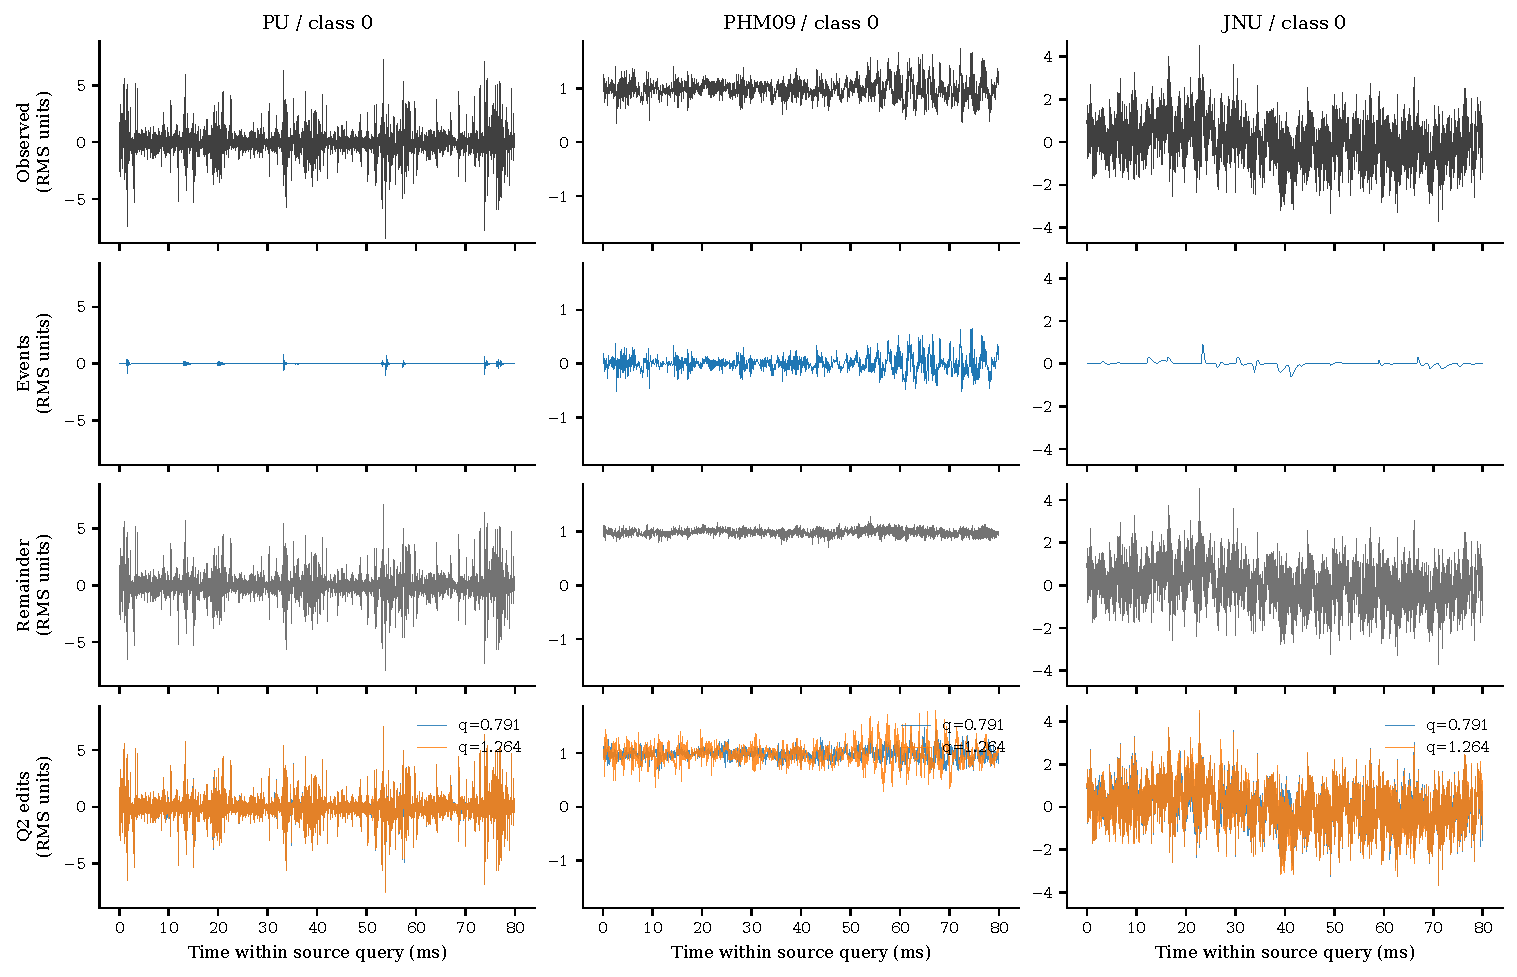
\includegraphics[width=.98\linewidth]{real_source_reference_examples.pdf}
\caption{Fixed class-0 source examples. PHM09 configuration 1 is not assumed to be a verified healthy reference. The within-column amplitude convention is the same as in Fig.~\ref{fig:source-edit}.}
\label{fig:reference-examples}
\end{figure}
\FloatBarrier
\begin{thebibliography}{99}

\bibitem{zhao2024}
C.~Zhao, E.~Zio and W.~Shen,
Domain generalization for cross-domain fault diagnosis: An application-oriented
perspective and a benchmark study,
Reliability Engineering \& System Safety 245 (2024) 109964.
\href{https://doi.org/10.1016/j.ress.2024.109964}{doi:10.1016/j.ress.2024.109964}.

\bibitem{chen2025}
Y.~Chen, D.~Zhang, R.~Yan and M.~Xie,
Applications of domain generalization to machine fault diagnosis: A survey,
IEEE/CAA Journal of Automatica Sinica 12(10) (2025) 1963--1984.
\href{https://doi.org/10.1109/JAS.2025.125120}{doi:10.1109/JAS.2025.125120}.

\bibitem{cis2n}
C.~Guo, Z.~Shang, J.~Ren, Z.~Zhao, B.~Ding, S.~Wang and X.~Chen,
CIS2N: Causal independence and sparse shift network for rotating machinery fault diagnosis in unseen domains,
Reliability Engineering \& System Safety 251 (2024) 110381.
\href{https://doi.org/10.1016/j.ress.2024.110381}{doi:10.1016/j.ress.2024.110381}.

\bibitem{pc3net}
N.~Jia, W.~Huang, C.~Ding, J.~Wang and Z.~Zhu,
PC3Net: A prior-causal contrast-collaboration network for single domain
generalization fault diagnosis,
Reliability Engineering \& System Safety 264 (2025) 111411.
\href{https://doi.org/10.1016/j.ress.2025.111411}{doi:10.1016/j.ress.2025.111411}.

\bibitem{antic2024}
G.~Zhang, X.~Kong, Q.~Wang, J.~Du, J.~Wang and H.~Ma,
Single domain generalization method based on anti-causal learning for rotating machinery fault diagnosis,
Reliability Engineering \& System Safety 250 (2024) 110252.
\href{https://doi.org/10.1016/j.ress.2024.110252}{doi:10.1016/j.ress.2024.110252}.

\bibitem{ccdg}
M.~Ragab, Z.~Chen, W.~Zhang, E.~Eldele, M.~Wu, C.-K.~Kwoh and X.~Li,
Conditional contrastive domain generalization for fault diagnosis,
IEEE Transactions on Instrumentation and Measurement 71 (2022) 3506912.
\href{https://doi.org/10.1109/TIM.2022.3154000}{doi:10.1109/TIM.2022.3154000}.

\bibitem{coral}
B.~Sun and K.~Saenko,
Deep CORAL: Correlation alignment for deep domain adaptation,
Computer Vision--ECCV 2016 Workshops, LNCS 9915 (2016) 443--450.
\href{https://doi.org/10.1007/978-3-319-49409-8_35}{doi:10.1007/978-3-319-49409-8\_35}.

\bibitem{dann}
Y.~Ganin, E.~Ustinova, H.~Ajakan, P.~Germain, H.~Larochelle, F.~Laviolette, M.~Marchand and V.~Lempitsky,
Domain-adversarial training of neural networks,
Journal of Machine Learning Research 17(59) (2016) 1--35.
\url{https://jmlr.org/papers/v17/15-239.html}.

\bibitem{cui2026}
J.~Cui, J.~Cheng, M.~Liu, Z.~Cheng and C.~Duan,
A two-stage semi-supervised domain generalization network for fault diagnosis under unknown working conditions,
Reliability Engineering \& System Safety 267 (2026) 111925.
\href{https://doi.org/10.1016/j.ress.2025.111925}{doi:10.1016/j.ress.2025.111925}.

\bibitem{mocd}
L.~Song, Z.~Lin, X.~Lu, M.~Zhang and H.~Wang,
A domain generalization fault diagnosis method based on matching optimization
and causal disentanglement,
Engineering Applications of Artificial Intelligence 179 (2026) 115151.
\href{https://doi.org/10.1016/j.engappai.2026.115151}{doi:10.1016/j.engappai.2026.115151}.

\bibitem{cfdcr}
M.~Jiang, K.~Zhou, J.~Gao and F.~Zhang,
Integrating causal representations with domain adaptation for fault diagnosis,
Reliability Engineering \& System Safety 260 (2025) 110999.
\href{https://doi.org/10.1016/j.ress.2025.110999}{doi:10.1016/j.ress.2025.110999}.

\bibitem{pang2024}
B.~Pang, Q.~Liu, Z.~Xu, Z.~Sun, Z.~Hao and Z.~Song,
Fault vibration model driven fault-aware domain generalization framework
for bearing fault diagnosis,
Advanced Engineering Informatics 62 (2024) 102620.
\href{https://doi.org/10.1016/j.aei.2024.102620}{doi:10.1016/j.aei.2024.102620}.

\bibitem{shi2024}
Z.~Shi, J.~Chen, Y.~Zi, K.~Cao and B.~Li,
Semi-physical simulation-driven contrastive decoupling net for intelligent
fault diagnosis of unseen machines under varying speed,
Measurement Science and Technology 35 (2024) 076101.
\href{https://doi.org/10.1088/1361-6501/ad36da}{doi:10.1088/1361-6501/ad36da}.

\bibitem{pcr2026}
Z.~Deng, N.~Hu, Y.~Yang, Z.~Yin, H.~Luo, X.~Lin, J.~Hao and Z.~Zhou,
Physics-guided counterfactual causal learning for explainable single-source
domain generalization cross-machine bearing fault diagnosis,
Advanced Engineering Informatics 69 (2026) 103955.
\href{https://doi.org/10.1016/j.aei.2025.103955}{doi:10.1016/j.aei.2025.103955}.

\bibitem{fista}
A.~Beck and M.~Teboulle,
A fast iterative shrinkage-thresholding algorithm for linear inverse problems,
SIAM Journal on Imaging Sciences 2(1) (2009) 183--202.
\href{https://doi.org/10.1137/080716542}{doi:10.1137/080716542}.

\bibitem{in}
D.~Ulyanov, A.~Vedaldi and V.~Lempitsky,
Instance normalization: The missing ingredient for fast stylization,
arXiv:1607.08022 (2016).

\bibitem{mixup}
H.~Zhang, M.~Cisse, Y.~N.~Dauphin and D.~Lopez-Paz,
mixup: Beyond empirical risk minimization,
International Conference on Learning Representations (2018).

\bibitem{pu}
C.~Lessmeier, J.~K.~Kimotho, D.~Zimmer and W.~Sextro,
Condition monitoring of bearing damage in electromechanical drive systems by
using motor current signals of electric motors: A benchmark data set for
data-driven classification,
PHM Society European Conference 3(1) (2016).
\href{https://doi.org/10.36001/phme.2016.v3i1.1577}{doi:10.36001/phme.2016.v3i1.1577}.

\bibitem{phm09}
PHM Society, 2009 PHM Society Conference Data Challenge: Gearbox data (2009).
\url{https://phmsociety.org/phm_competition/2009-phm-society-conference-data-challenge/}.

\bibitem{jnu}
Jiangnan University bearing dataset,
\href{https://github.com/ClarkGableWang/JNU-Bearing-Dataset}{public distribution repository}
(accessed 29 October 2026).
\end{thebibliography}

\end{document}
